\newif\ifdraft\drafttrue  % set true to show comments
\newif\iflastminute\lastminutefalse  % for things to check at the end

\documentclass[acmsmall,review,anonymous]{acmart}
\settopmatter{printfolios=true,printccs=false,printacmref=false}
% % For double-blind review submission, w/ CCS and ACM Reference
% \documentclass[acmsmall,review,anonymous]{acmart}\settopmatter{printfolios=true}
% % For single-blind review submission, w/o CCS and ACM Reference (max
% submission space)
% \documentclass[acmsmall,review]{acmart}\settopmatter{printfolios=true,printccs=false,printacmref=false}
% % For single-blind review submission, w/ CCS and ACM Reference
% \documentclass[acmsmall,review]{acmart}\settopmatter{printfolios=true} % For
% final camera-ready submission, w/ required CCS and ACM Reference
% \documentclass[acmsmall]{acmart}\settopmatter{}


% % Journal information % Supplied to authors by publisher for camera-ready
% submission; % use defaults for review submission.
\acmJournal{PACMPL}
\acmVolume{1}
\acmNumber{ICFP} % CONF = POPL or ICFP or OOPSLA
\acmArticle{1}
\acmYear{2018}
\acmMonth{1}
\acmDOI{} % \acmDOI{10.1145/nnnnnnn.nnnnnnn}
\startPage{1}

% % Copyright information % Supplied to authors (based on authors' rights
% management selection; % see authors.acm.org) by publisher for camera-ready
% submission; % use 'none' for review submission.
\setcopyright{none}
\usepackage{algorithm, amsmath, amssymb, verbatim, enumerate, graphicx,
  centernot, tikz, array, mathtools, bussproofs, stmaryrd, enumitem,
  stackengine, subcaption, cleveref}
\captionsetup{compatibility=false}
\usepackage{relsize}
\usepackage{listings}
\usepackage{proof}
\usepackage{xspace}
\usepackage[noend]{algpseudocode}

\lstset{ language=Caml, basicstyle=\linespread{0.8}\upshape\sffamily,
keywordstyle=\upshape\sffamily\color{dkblue}, keepspaces=true,
framexleftmargin=1ex, framexrightmargin=1ex, showstringspaces=true,
commentstyle=\itshape\rmfamily,
emph={synth,project,perm,squash,normalize,using,ins,del,lens,let},
emphstyle=\upshape\sffamily\color{dkred}, 
columns=fullflexible,
escapechar=\#,
% BCP: I find this distracting:
% stringstyle=\sffamily\color{dkred},
mathescape, }

% %%%% Macros Colors
\definecolor{dkblue}{rgb}{0,0.1,0.5}
\definecolor{dkgreen}{rgb}{0,0.6,0}
\definecolor{dkred}{rgb}{0.6,0,0}
\definecolor{dkpurple}{rgb}{0.7,0,0.4}
\definecolor{olive}{rgb}{0.4, 0.4, 0.0}
\definecolor{teal}{rgb}{0.0,0.5,0.5}
\definecolor{orange}{rgb}{0.9,0.6,0.2}
\definecolor{lightyellow}{RGB}{255, 255, 179}
\definecolor{lightgreen}{RGB}{170, 255, 220}
\definecolor{teal}{RGB}{141,211,199}
\definecolor{darkbrown}{RGB}{121,37,0}

\newcommand{\FINISH}[3]{\ifdraft\textcolor{#1}{[#2: #3]}\fi}
\newcommand{\bcp}[1]{\FINISH{dkred}{B}{#1}}
\newcommand{\BCP}[1]{\FINISH{dkred}{B}{\bf #1}}
\newcommand{\afm}[1]{\FINISH{dkgreen}{A}{#1}}
\newcommand{\dpw}[1]{\FINISH{dkblue}{D}{#1}} % Toronto Maple Leafs Blue :-)
\newcommand{\saz}[1]{\FINISH{orange}{SZ}{#1}}
\newcommand{\SAZ}[1]{\FINISH{orange}{SZ}{#1}}
\newcommand{\ksf}[1]{\FINISH{teal}{K}{#1}}
\newcommand{\sam}[1]{\FINISH{dkpurple}{SM}{#1}}

% For Inference Rules
\newcommand{\Rule}[2]{\infer{#2}{#1}}
\newcommand{\RuleSide}[3]{\infer[#3]{#2}{#1}}
% \newcommand{\Axiom}[1]{\Rule{}{#1}}

\newcommand{\wf}[1]{\ensuremath{#1\;\mathsf{wf}}}

% FOR Regular Expression names
\newcommand{\re}[1]{\ensuremath{\mathtt{#1}}}
\newcommand{\codefont}[1]{\ensuremath{\mathsf{#1}}}
\newcommand{\kw}[1]{\codefont{#1}}
\newcommand{\project}[2]{\ensuremath{\kw{project} \; #1 \mapsto #2}}
\newcommand{\squash}[3]{\ensuremath{\kw{squash} \; #1 \rightarrow #2\; \kw{using} \; #3}}
\newcommand{\perm}[2]{\ensuremath{\kw{perm}\; (#1)\; \kw{with}\; #2}}
\newcommand{\normalize}[3]{\ensuremath{\kw{normalize}(#1, #2, #3)}}
\newcommand{\eqrel}[1]{\ensuremath{\equiv_{#1}}}
\newcommand{\sep}{\ensuremath{\ | \ }}
\newcommand{\canonize}{\ensuremath{\kw{canonize}}}
\newcommand{\bibtex}{\textsc{Bib}\TeX{}}
\newcommand{\get}{\ensuremath{\kw{get}}}
\newcommand{\semicolon}{\ensuremath{\; ; \;}}
\newcommand{\lput}{\ensuremath{\kw{put}}}
\newcommand{\create}{\ensuremath{\kw{create}}}
\newcommand{\const}{\ensuremath{\kw{const}}}
\newcommand{\swap}{\ensuremath{\kw{swap}}}
\newcommand{\id}{\ensuremath{\kw{id}}}
\newcommand{\lquot}{\ensuremath{\kw{lquot}}}
\newcommand{\rquot}{\ensuremath{\kw{rquot}}}
\newcommand{\lift}{\ensuremath{\kw{lift}}}


\newcommand{\Name}{Optometrist\xspace}

\newcommand{\QRESize}{\textbf{QS}}
\newcommand{\canonizeAndSpecSize}{\textbf{CS}}
\newcommand{\LensAndSpecSize}{\textbf{LS}}

\newcommand{\OpticianRuntime}{\textbf{OO}}
\newcommand{\SystemOnOptician}{\textbf{QO}}
\newcommand{\SystemOnBenchmarks}{\textbf{QQ}}
\newcommand{\cd}[1]{\lstinline[backgroundcolor=\color{white}]$#1$}


% %%%%%%%%%%%%%%%%%%%%%%%%%%%%%%%%%%

\begin{document}
\title{Synthesizing Quotient Lenses}
\begin{abstract}
{\em Quotient lenses} are bidirectional transformations whose correctness
laws are ``loosened'' by specified equivalence relations, allowing
inessential details in concrete data formats to be suppressed. 
For example, a programmer could use a quotient lens to define 
a transformation that ignores the order of fields in XML data, so
that two XML files with the same fields but in different orders would be
considered the same, allowing a single, simple lens to handle them both. 

We offer three interconnected innovations to simplify the task of programming
quotient lenses.  
First, we introduce {\em quotient regular expressions} (QREs), to
easily mark aspects of data formats that are
inessential.  A QRE is an augmented regular expression that
simultaneously defines a regular language and an equivalence
relation on this language.  Variations within the same
equivalence class are deemed inessential. 
Next, we introduce {\em QRE lenses}, i.e., lenses mapping
between QREs.
Our key technical result is a proof that every QRE lens can be
transformed into one of the form $c_1 ; \ell ;
c_2^{-1}$, where $c_1$ and $c_2^{-1}$ are {\em canonizers}, $\ell$ is a bijective
transformation, and $;$ is composition\iflastminute\bcp{$c_2^{-1}$ is ugly, but I think
  we need the superscript for accuracy.  Perhaps calling them $c$ and $d$
  instead of $c_1$ and $c_2$ would be better?}\fi.  Intuitively,
the canonizers normalize data by picking a
canonical representative of the relevant equivalence relations. 
This theorem means we can push all normalization to the outer edges of a
bidirectional transformation, leaving in the middle a pure bijective
transformation.  
Finally,
we leverage this normalization theorem to {\em synthesize} QRE lenses from a pair
of QREs and example input-output pairs, reusing earlier work on
synthesizing plain bijective lenses.
We have implemented QREs and QRE lens synthesis 
in the bidirectional programming language Boomerang.
We evaluate the effectiveness of our approach by using it to
synthesize QRE lenses between various real-world data formats in
the Optician benchmark suite.

\end{abstract}

\keywords{quotient regular expressions, QRE lens, synthesis}
\maketitle

\section{Introduction}
Often, the same data is stored in more than one format. For example,
bibliographic data may be stored in \bibtex{} or EndNote formats,
spreadsheet data can be represented as either CSV and TSV files, and web
APIs can return data as either JSON or XML objects.  When changes are
made one version, the data in the other must be updated so the
two continue to represent the same information.
One way to synchronize such data is to use \emph{lenses}~\cite{Lenses}, 
programs that simultaneously define pairs of functions for translating
the data from the source format to the target formant (the \emph{get}
direction) and back again (the \emph{put} direction). Lenses can be
written in one of several domain-specific bidirectional languages that 
guarantee various \emph{lens laws} constraining how the \emph{put} and
\emph{get} functions must fit together. 

\emph{Bijective lenses} are amongst the most restrictive. 
A bijective lens $\ell : S \Leftrightarrow T$ specifies a bijection from
a source set $S$ to a target set $T$:
\begin{equation}\label{bijectivelenslaws}
\ell.\get \; (\ell.\lput \; t) = t \text{, and } \ell.\lput \; (\ell.\get \; s)
= s
\end{equation}
Since the \emph{get} and \emph{put} functions form a bijection, 
no information is lost during translation from one data format to another. 
While this very strong guarantee can sometimes be useful, it is more common for 
some of the details in one or both of the data formats to be
superfluous. For instance, the number of white space characters
between data items, the capitalization of various strings, the
sequence of fields in a record, or the order of items in a list are
often irrelevant.  Also, many
data formats introduce their own ad hoc conventions about formatting details
that are taken to be inessential. In \bibtex{}, for example,
an author can be specified either as 
``\cd{lastname, firstname}'' or as ``\cd{firstname lastname}''.

{\em Quotient lenses}~\cite{quotientlenses} loosen the strong restrictions of
bijective string lenses by including equivalence
relations on the source and target formats and requiring that the
round-tripping lens laws 
hold  modulo these equivalences, rather than ``on the nose.'' Quotient lenses 
make it possible to synchronize many more data formats than is possible with
plain bijective lenses\bcp{Do we justify this claim later?}. 

The bidirectional programming language {\em
Boomerang}~\cite{boomerang} is the only language we know of that
implements a general class of quotient lenses.  Unfortunately, these
lenses to have two main drawbacks.  

The first drawback is that defining an equivalence
relation in Boomerang requires specifying a {\em canonizer}, which is
a pair of functions $f$ and $g$ where $f$
normalizes data from the
external format by choosing canonical representations
and $g$ provides an
inverse by specifying the external form of each canonical
representation. 
The disadvantage of this approach is that writing
a quotient lens in Boomerang requires defining four
different data formats: two ``external'' formats which specify the data to
be transformed by the lens, and two ``internal'' formats which specify the
canonical representations for the source and target data.

Our solution to this shortcoming is to introduce {\em Quotient Regular
Expressions} (QREs), which enable programmers to simultaneously specify a
regular expression and a set of canonical representatives for matching
strings.  Given an QRE, we can automatically infer the corresponding
canonization functions.  As an example, consider the following QRE for writing
author names:
\iflastminute
\bcp{I'd love to use a visible space symbol for important space characters
  -- this would make the code examples very much clearer!  But it will
  require a bit of hacking: We can use showstringspaces=false}
\fi
%
\begin{lstlisting}
let wsp_sp = project wsp $\to$ " "
let comma_name = first_name . "," . wsp_sp . last_name
\end{lstlisting}
%
In this example, \lstinline{wsp} is an existing regular expression for a
nonempty sequence of whitespace characters, and \lstinline{first_name} and
\lstinline{last_name} are existing regular expressions for first and last names.
The QRE \lstinline{wsp_sp} is a QRE with the same underlying language as
\lstinline{wsp}, but with a single canonical representative: \lstinline{" "}.
This is then used to build up \lstinline{comma_name}, a QRE with an
underlying language of two names, separated by a command and whitespace, where
the names with a single space between them are canonical.

The second drawback with writing quotient lenses in Boomerang is that
even after specifying the four required data formats, the programmer must
still define a lens for converting between the canonical
representations.   Experience shows that writing such lenses can be
tedious (consider having to rearrange the order of data items by recursively
using operators to \kw{swap} adjacent fields)  and that satisfying the type
checker can be difficult because many seemingly useful lenses contain
ambiguities disallowed by the Boomerang type checker~\cite{optician}.

Our solution to this problem is to introduce {\em QRE lenses}, which
are a new class of quotient lens that can be automatically
synthesized, obviating the need to write lenses by hand.  A QRE lens
is like a normal lens except it maps between formats described by
QREs. We prove a normal form theorem (Theorem~\ref{normal form}) that says that
every composition of QRE lenses can be rewritten 
to be the composition of a source canonizer, a bijective lens, and a
target canonizer. This normalization property means we can synthesize
QRE lenses by extending an existing algorithm for synthesizing
bijective lenses~\cite{optician}.  

Given this framework, generating a QRE lens requires only a pair of QREs to describe the
source and target formats and a (possibly empty) suite of examples
demonstrating the mapping.  For example, the following code

\begin{lstlisting}
let l = synth comma_name $\Leftrightarrow$ space_name using {("Lovelace, Ada", "Ada Lovelace")}
\end{lstlisting}
binds \codefont{l} to a synthesized QRE lens mapping between names in
the comma-separated form describd by the QRE \codefont{comma\_name}
and the space-separated form described by the
QRE \codefont{space\_name}. 
The lenses generated by
our synthesis algorithm are guaranteed to translate data back and forth
between source and target QREs and to satisfy the provided examples.
Our synthesized quotient lenses have a relatively
restricted form (which greatly speeds up synthesis), but the 
normalization theorem means 
this restriction does not compromise expressiveness.

The following list summarizes the contributions of our work.
\begin{enumerate}
  \item We introduce {\em Quotient Regular Expressions} (QREs), which are
  a compact, convenient notation for simultaneously defining a
  regular language modulo some equivalence relation and a canonizer
  for that relation (Section~\ref{QRE}).
  \item We introduce {\em QRE lenses}, which are lenses that translate
  between data formats specified using QREs. (Section~\ref{QRE-lenses}).
  \item We descibe a particular set of QRE lens combinators and prove
  that QRE lenses defined using these combinators can be normalized
  (Theorem~\ref{normal form}), which is the main technical
  contribution of this paper.
  (Section~\ref{QRE-lenses}).
  \item We use this result to reduce the problem of {\em synthesizing} QRE
  lenses to the problem of synthesizing bijective string lenses
  previously studied in~\cite{optician}(Section~\ref{synth}).
  \item We extend Boomerang with QREs and QRE lens synthesis. 
  We use the resulting implementation to demonstrate the utility of
  our approach by synthesizing QRE lenses between
  data formats drawn from the Optician benchmark suite (Section~\ref{impl}).
\end{enumerate}
Sections~\ref{relwork} and~\ref{concl} discuss related and future work.

\section{Background: Bijective String Languages}
\label{sec:background}
\iflastminute
\ksf{We are inconsistent in how we typeset get/put.  Sometimes we use
codefont, sometimes we use italics of various flavors, and sometimes
we don't do anything distinctive.  It would be good to be consistent!}
\fi
Before describing QREs and QRE lenses, we briefly review bijective
string lenses. Consider a bidirectional transformation that converts
between \bibtex{} citation records such as
\begin{verbatim}
  @Book {Lovelace,
  Author = "Ada Lovelace",
  Title = {Notes}
}
\end{verbatim}
\noindent
and equivalent EndNote records like the following
\begin{verbatim}
  %0 Book
  %F Lovelace
  %A Ada Lovelace
  %T Notes
\end{verbatim}
\noindent
Boomerang's bijective string lenses are designed to define bidirectional
transformations such as this one, where the data formats can be matched in a
one-to-one manner, in this case by matching the label, author and title fields.
Boomerang encourages a compositional approach in which programmers
define simple lenses and then compose them using a variety of
combinators. 

Primitive lenses include:
\begin{itemize}
  \item \kw{del} $s$: delete the constant string $s$ in the get
  direction; insert it in the put direction.
  \item \kw{ins} $s$: insert the constant string $s$ in the get
  direction; delete it in the put direction.
  \item \kw{copy} $R$: copy the text matching the regular expression $R$ in
  both directions.
\end{itemize}
Such primitives may be combined using the regular operators
Kleene star, alternation and concatenation, as well as lens composition.
Figure~\ref{fig:example-lens} illustrates the use of these
combinators to define a lens \cd{bib_to_end} that transforms data
in \bibtex{} to EndNote (and vice versa). 
\begin{figure}[t]
\begin{lstlisting}
let preamble : "@book{" $\Leftrightarrow$ "%0 Book\n%F " =
del "@book{" . ins "%0 Book\n%F "

let author_lens : (",\n" . bib_author) $\Leftrightarrow$ ("\n" . end_author) =
del ",\nauthor = \""
. ins "\n%A "
. name
. (del " and "
. ins "\n"
. (ins "%A " . name . del " and " . ins "\n")*
. ins "%A "
. name
|| "")

let title_lens : ("\",\n" . bib_title . "},\n}") $\Leftrightarrow$ ("\n" . end_title) =
del "\",\ntitle = {" . ins "\n%T " . title . del "},\n}"

let bib_to_end : bibtex $\Leftrightarrow$ end_note = preamble . label . author_lens . title_lens
\end{lstlisting}
\caption{An example bijective lens \cd{bib_to_end} between data
matching \cd{bibtex} and \cd{end_note} regular 
expressions, which are omitted for brevity.  
\iflastminute
\bcp{a possible readability suggestion: define a named constant for a quote
  character.  (Not sure if this makes sense, or if it improves things...)}
\fi}
\label{fig:example-lens}
\end{figure}

Recent work described the {\em Optician}
algorithm/tool~\cite{optician}, which can synthesize bijective lenses
such as \cd{bib_to_end}, obviating the sometimes tedious tasks
involved in writing such lenses by hand.  Given the directive
\begin{lstlisting}
synth S <=> T using exs
\end{lstlisting}
\noindent
{\em Optician} will synthesize a bijective lens between 
source and target formats described by regular expressions
\cd{S} and \cd{T}, respectively, and a set of input-output example pairs \cd{exs} specifying how
the synthesized lens should behave on those examples.


\section{QRE Lenses by Example}
\label{sec:example}

{\em Optician} greatly simplifies the task of programming bijective
string lenses, but not all bidirectional transformations are
bijective.  For instance, \bibtex{} users are not typically interested
in preserving whitespace between words.  The order of author and title
fields is also likely irrelevant, and there may be equivalent ways of
writing the same name: ``Lovelace, Ada'' vs ``Ada Lovelace.''
Consequently, the following two \bibtex{} citations represent the same
logical object even though they differ in nonessential details.
\begin{verbatim}
@Book {Lovelace,
Author = "Ada Lovelace",
Title = {Notes},
}

@Book{     Lovelace,
Title = {Notes},
Author = "Lovelace, Ada",     }
\end{verbatim}

When mapping these records into another format, such as EndNote, we
must decide what to do with the nonessential information.  A bijective
mapping must preserve all the information, including the extraneous
details, which leads to complex and brittle lenses complicated by the
need to preserve unimportant details.  
A better approach is to identify records that differ only in the
nonessential information, mapping them into a canonical representation.
This canonical representation is then mapped into the target format.
With this approach, both of the above \bibtex{} records would be
mapped to the same EndNote record.

We use {\em Quotient Regular Expresions} (QREs) to specify the
external format in full detail and to mark which pieces of it are
inessential.  From a QRE, we can infer a regular expression that
describes only the essential information, which we call the internal
format, and we can derive a canonizer that maps between the external
and internal formats.


\subsection{Specifying \bibtex{} Using QREs}
\label{subsec:qre-expressions}
\ksf{Are these QRE combinators or QRE lens combinators?  
We are currently mushy about this distinction.  
The section needs a pass to clarify this point.
The headers of this section and the next imply that this section is
about QREs and the next section is about QRE lenses, but this section
is where we introduce the QRE lens combinators, right?  If so, we need
to do something to make the structure clearer.}\afm{I believe this are QRE
combinators, so we should be good.}

In this subsection, we develop a QRE specification of \bibtex{}
records, introducing various QRE combinators along the way. 
Our first step in this process is to define a
whitespace format, which externally matches any non-zero number of whitespace
characters. It converts any such whitespace into a single space
character, its canonical form. 
We use the QRE \kw{project} primitive to define this
whitespace-normalizing QRE. \bcp{Why is it called
``project''?} \ksf{select seems like it might be a better name as we
are choosing one representative element from a set of possibilities.}\bcp{Or
``collapse''?}

\begin{lstlisting}
let wsp_sp = project wsp $\to$ " "
\end{lstlisting}
\iflastminute
\bcp{Can we display blanks as a distinct ``visible blank'' symbol
(throughout)?  That will make examples easier to read.}\bcp{I tried turning
on the showstringspaces option at the top, but that doesn't do everything we
want--it only works inside quotes.  But the latex ``textvisiblespace'' command
produces a single one, and the lstlisting ``escapechar'' option will allow
us to use it inside listings.  But we should save this for the final
tweaking stage.}\bcp{Done, I think.}
% Here is an example: if you set escapechar=\%, you could use it inside the
% listings as follows: \begin{lstlisting} t %\leftarrow% 0 \end{lstlisting}
\fi

Sometimes there are multiple disjoint representations of the same data.
In such situations, the QRE \kw{squash} combinator creates a QRE that
allows external data to be in either format, and converts any
data in the first format to the second.
For instance, assume that
the \codefont{comma\_name} format describes ``Lovelace, Ada''
and that the \codefont{space\_name} format describes ``Ada Lovelace''
and \codefont{c\_to\_s} is a function from the first to the second.  In this
case, the following instance of \kw{squash} creates the desired canonizer.

%Figure~\ref{fig:example-qre} illustrates
%how to specify \bibtex{} records and their canonical elements using
%QREs.

\begin{lstlisting}
let name = squash comma_name $\to$ space_name using c_to_s
\end{lstlisting}

One way to define the \codefont{c\_to\_s} function
is simply to write it from scratch in some ordinary programming language.
However, we can synthesize such functions automatically---here, \codefont{c\_to\_s} is the
\codefont{get} direction of a lens that can be synthesized using the 
\kw{synth} combinator:
%
\begin{lstlisting}
let l = synth comma_name $\Leftrightarrow$ space_name using {("Lovelace, Ada", "Ada Lovelace")}
let c_to_s = get l
\end{lstlisting}
\noindent
The first line above synthesizes a lens between \codefont{comma\_name} and
\codefont{space\_name} using the listed example transformation as a guide.  The
second line extracts the \codefont{get} direction transformation from the lens,
which is what we need for \kw{squash}.

The permutation QRE combinator, \kw{perm}, allows data to be unordered. For example,
the following instance of \kw{perm} allows label, author and title fields
(which we assume have been defined earlier) to appear in any order.
%
\begin{lstlisting}
let bib_fields = perm (label, bib_author, bib_title)
\end{lstlisting}
%
To normalize the field separators, one can specify 
in an optional \kw{with} clause that the components of the
permutation are conjoined by another QRE. For instance, below, we normalize
whitespace between fields, leaving only a single newline.
%
\begin{lstlisting}
let bib_fields = perm (label, bib_author, bib_title) with (project ("," . wsp) $\to$ ",\n")
\end{lstlisting}

Another QRE primitive is the sequential composition combinator, written ``;''.
For an example of its use, suppose we have already defined a QRE,
\lstinline{canonized_whitespace}, that accepts XML documents and chooses
documents with no whitespace as canonical. Suppose that we also have defined a
QRE, \lstinline{canonized_order}, which accepts whitespace-normalized XML
documents, and chooses a specific ordering of XML elements as canonical. We can
use the sequential composition combinator to combine these two QREs into
\lstinline{canonized_whitespace ; canonized_order}, a QRE that accepts all XML
documents, and chooses ordered XML documents without whitespace as canonical.

The final QRE combinator is the \kw{normalize} combinator. This combinator
allows a programmer to manually define a function $f$ which sends each
string that matches a regular expression $R$ to some canonical
representative in another regular expression $R'$. The equivalence
relation defined by the normalize combinator is hence the equivalence
relation defined by the {\em fibres} of $f$; that is, for all strings
$s$ and $s'$ that match $R$, $s$ is equivalent to $s'$ if and only if
$f(s) = f(s')$.

For instance, assume that $f(s)=$ ``\textvisiblespace'' (a space
character) for all whitespace strings $s$. Then the 
project QRE \lstinline{wsp_sp} defined above can
be expressed using the normalize combinator as
\lstinline{normalize (wsp," ", f)}.

Figure~\ref{fig:example-qre} gives the complete QRE specification for the
\bibtex{}.
\begin{figure}
\begin{lstlisting}
let wsp = [#\,\textvisiblespace\,#\n\t\r]+
let wsp_sp = project wsp $\to$ " "
let last_name = [A-Z][a-z]
let first_name = [A-Z][a-z]

(* define name representations with a space and with a comma *)
let space_name = first_name . wsp_sp . last_name
let comma_name = last_name . "," . wsp_sp . first_name

(* synthesize a lens that maps comma representation to space representation *)
let l = synth comma_name $\Leftrightarrow$ space_name using {("Lovelace, Ada", "Ada Lovelace")}
let c_to_s = get l

(* squash QRE maps comma_name to space_name *)
let name = squash comma_name $\to$ space_name using c_to_s

(* define rest of bibtex fields *)
let bib_names = name . (wsp_sp . "and" . wsp_sp . name)$^*$
let bib_author = "author = \"" . bib_names . "\""
let title = word . (wsp_sp . word)$^*$
let bib_title = "title = {" . title . "}"

(* allow any permutation of fields interspersed with arbitrary whitespace *)
let bib_fields = perm (label, bib_author, bib_title) with (project ("," . wsp) $\to$ ",\n")
let bibtex = "@book{" . bib_fields . "}"
\end{lstlisting}
\caption{QRE specification of \bibtex{} records.\ksf{In what sense is this a QRE
spec vs a QRE lens spec?}}
\label{fig:example-qre}
\end{figure}


\subsection{QRE Lenses and QRE Lens Synthesis}
\label{sec:examplesynth}
At this point we have a tool for synthesizing bijective string lenses from a
pair of regular expressions and a set of example input-output pairs
({\em Optician}), 
and we have a way of defining regular expressions with equivalence
relations indicating the essential information (QREs).
A tantalyzing possibility would be to use the bijective string lens
synthesis procedure as a subroutine for a quotient lens synthesis procedure. 
This new synthesizer would take as input source and target QREs and 
example input-output pairs, 
compute the canonical source/target formats from the QREs, 
map the example input-output pairs to their canonical representations,
and then invoke the bijective string lens synthesis procedure on the canonical data
formats and the canonical examples.

Indeed this idea is what motivates our definition of {\em QRE lenses}.
Intuitively, our QRE lenses are bijective lenses with ``canonizers at the edges,''
just like Boomerang's quotient lenses. 
Figure~\ref{fig:attheedges} depicts the architecture of QRE lenses.
\begin{figure}[t]
\centering
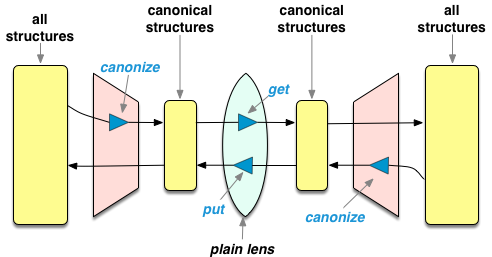
\includegraphics[width=0.7\textwidth]{canonizers-outside}
\caption{QRE Lens with ``Canonizers at the Edges''}
\label{fig:attheedges}
\end{figure}
Every QRE lens $q_1$ has a type $q_1: Q_1 \Leftrightarrow Q_2$ where $Q_1$ and $Q_2$
are QREs. In the {\em get} direction, a QRE lens $q_1: Q_1 \Leftrightarrow Q_2$ uses the
source QRE $Q_1$ to compute a canonical representative for the data modulo the
equivalence relation defined by $Q_1$ and then applies the $\get$ function of a
bijective string lens $\ell_1$ to this representative. In the {\em put} direction, $q_1$
operates similarly, but using the QRE $Q_2$ and the $\lput$ function of
$\ell_1$.

Because the QREs $Q_1$ and $Q_2$ determine the internal formats for data after
canonization, and because the algorithm for synthesizing bijective string lenses is
directed by these formats, $Q_1$ and $Q_2$ are all that is required to
synthesize QRE lenses end-to-end. 

However, our restriction that canonizers appear only at the edges
raises a key technical question: Are we limiting the expressiveness of
our transformations by demanding all programs fit into this normal
form?  It turns out that we are not: any lens that uses canonizers
internally can be transformed into a lens that uses canonizers only at
the edges. The main technical contribution of this paper
(Theorem~\ref{normal form})
is a proof of this fact.
This technical result justifies 
using synthesis to produce QRE lenses instead of manually writing
them,
which can lead to substantial savings in program complexity.
For instance, after defining the \bibtex{} and EndNote QREs and
binding them to the variables \cd{bibtex} and \cd{endnote} respectively, then
all the code in Figure~\ref{fig:example-lens} may be replaced by a single call
to the synthesis prodedure:
\begin{lstlisting}
let bib_to_end : bibtex $\Leftrightarrow$ endnote =
synth bibtex $\Leftrightarrow$ endnote using {(bib_example, end_example)}
\end{lstlisting}
\noindent 
Here, the generated quotient lens synchronizes \cd{bibtex} and
\cd{endnote} formats, using \cd{bib_example} and \cd{end_example} (the two
concrete example strings given at the beginning of this section) to
disambiguate. In addition, and as we saw earlier with the definition of
\cd{c_to_s}, the synthesis procedure itself can be used to create lenses that
are in turn used to define other QREs.  The ability to interleave QRE
specification with QRE lens synthesis yields a powerful and flexible way of
creating bidirectional transformations.

\section{Quotient Regular Expressions}
\label{QRE}
A Quotient Regular Expression (or QRE) is a regular expression $R$ augmented
with syntax that expresses an equivalence relation on the language of $R$. This
section describes in further detail the set of QRE combinators that we described
in \cref{sec:example}.
\iflastminute 
\saz{Why does the ``cref'' macro not capitalize Section?}
\bcp{Dunno.  Because SIGPLAN does not want it to??  But maybe we should be
  using autoref instead anyway...}
\fi

\subsection{Syntax of Semantics of QREs}
Formally, the language of Quotient Regular Expressions (QREs) is given by the
following grammar:
\newcommand{\bsep}{\ \ \sep{} \ \ }
\begin{align*}
Q := \; & \normalize{R}{R'}{f} \bsep{} \id(R) \bsep \project{R}{s} \bsep \squash{Q_1}{Q_2}{f} \\
 | \; & \perm{Q_1, \ldots, Q_n}{Q} \bsep Q_1 \semicolon Q_2 \bsep Q_1 \cdot Q_2 \bsep (Q_1
\sep Q_2) \bsep Q^*,
\end{align*}
where $Q$ ranges over QREs, $R$ ranges over regular expressions, $f$ ranges over
functions between regular languages, and $s$ ranges over character strings.

Using the conventional notation that $\mathcal{L}(R)$ is the language accepted
by the regular expression $R$, each QRE $Q$ enables us to express four semantic objects

\begin{tabular}{rl}
  $W(Q)$  & a regular expression (the ``whole'' of $Q$),\\
  $\eqrel{Q}$  & an equivalence relation on $\mathcal{L}(W(Q))$,\\
  $K(Q)$ & a regular expression (the ``kernel'' of $Q$) such that
           $\mathcal{L}(K(Q))$ forms a complete \\
             & set of representatives for $\eqrel{Q}$, and \\
  $\canonize(Q)$ & 
  a ``canonizing'' function that, given any $w \in \mathcal{L}(W(Q))$,
  yields $\canonize(Q)(w)$ \\ & as the unique $k$ in $\mathcal{L}(K(Q))$ such
  that $k$ is equivalent to $w$ mod $\eqrel{Q}$
\end{tabular}
  % of type $\mathcal{L}(W(Q)) \longrightarrow \mathcal{L}(K(Q))$  which

The well-formedness constraints for QREs ensure that these four semantic
components fit together to form a coherent quotient $W(Q)/\eqrel{Q}$ whose
equivalence classes are determined by \canonize(Q).

\subsection{The \kw{normalize} Combinator}

The relationship among the semantic objects of a QRE can be understood in terms
of the \normalize{R}{S}{f} combinator, which exposes each of these pieces
explicitly.  Its whole language is just $R$, its kernel language is just
$S$, and $\canonize(\normalize{R}{S}{f}) = f$.  Its equivalence relation is
determined by the fibres of $f$, so we have
$s_1 \equiv s_2 \Leftrightarrow f(s_1) = f(s_2)$.

These components form a coherent quotient language when the canonization
function $f$ is surjective and idempotent (intuitively, $f$ picks out a unique
representative for each equivalence class).  We also require that the kernel
language be a subset of the whole language, which enables QRE composition.
These considerations lead to the following well-formedness rule.

\begin{prooftree}
\AxiomC{$\mathcal{L}(S) \subseteq \mathcal{L}(R)$}
\AxiomC{$f : \mathcal{L}(R) \longrightarrow \mathcal{L}(S)$}
\AxiomC{$f$ is surjective}
\AxiomC{$f = f^2$}
\RightLabel{(Normalize)}
\QuaternaryInfC{$\wf{\normalize{R}{R'}{f}}$}
\end{prooftree}

Semantically, the \kw{normalize} QRE is universal---each of the other
combinators $Q$ is equivalent to $\normalize{W(Q)}{K(Q)}{f}$ for some
surjective, idempotent function
$f : \mathcal{L}(W(Q)) \longrightarrow \mathcal{L}(K(Q))$.   However,
although \kw{normalize} is powerful, verifying that a canonization function $f$
is surjective and idempotent is in general undecidable.  This means that a
programmer wishing to use \kw{normalize} must discharge strong proof
obligations, which is cumbersome in practice.\footnote{In our implementation we allow a programmer to use \kw{normalize} at their
own risk without checking these side conditions as an ``escape hatch'' for the
case when other QRE combinators are insufficient.\bcp{Do we use this in any
  of the programs we've written?}}

The remaining QRE combinators provide simpler, more compositional ways of
building canonizers.  Nevertheless, the \kw{normalize} combinator gives a
sufficient condition for potential QREs to be well-behaved, particularly with
respect to the strategy for synthesizing quotient lenses which we shall
introduce in Section~\ref{synth}, so we use it to guide the design of our QRE
combinators, as we see next.

% ; this is the second
% property that distinguishes the \kw{normalize} combinator from the other QREs.
% The \kw{normalize} combinator is special in two main ways, the first of 
% which has to do with the premises in its inference rule:


\subsection{QRE Combinator Semantics}

Figure~\ref{fig:wk} gives the inductive definitions of the whole and
kernel languages $W(Q)$ and $K(Q)$ for all of the QRE forms.
\begin{figure}[t]
\centering
\[
\begin{array}{l@{\quad}l@{\quad}l}

Q & W(Q) & K(Q) \\ \hline
R & R & R \\
\project{R}{s} & R & s \\
\squash{Q}{Q_1}{f} & W(Q) \sep W(Q_1) & K(Q_1) \\
\normalize{R}{R'}{f} & R & R' \\
Q_1 \; ; \; Q_2 & W(Q_1) & K(Q_2) \\
Q_1 \cdot Q_2 & W(Q_1) \cdot W(Q_2) & K(Q_1) \cdot K(Q_2) \\
Q_1 \sep Q_2 & W(Q_1) \sep W(Q_2) & K(Q_1) \sep K(Q_2) \\
Q^* & W(Q)^* & K(Q)^* \\
\end{array}
\]
\[
\begin{array}{r@{\quad}l}
W( \perm{Q_1, \ldots, Q_n}{Q} ) = &
\bigcup \limits_{\sigma \in S_n} W(c_{\sigma(1)}) \cdot W(Q) \cdot \ldots \cdot
W(Q) \cdot W(c_{\sigma(n)})\\
K( \perm{Q_1, \ldots, Q_n}{Q} ) = & K(Q_1) \cdot K(Q) \cdot \ldots \cdot K(Q)
\cdot K(Q_n)
\end{array}
\]
\caption{Whole and Kernel Regular Expressions}
\label{fig:wk}
\end{figure}
The \kw{squash} and \kw{permutation} combinators have the two most
interesting definitions. If $Q = \squash{Q_1}{Q_2}{f}$, then the whole language
of $Q$ is $W(Q_1) \sep W(Q_2)$. This is because the \kw{squash} combinator
takes the whole language $W(Q_1)$ of $Q_1$, the whole language $W(Q_2)$ of $Q_2$
and a function $f : \mathcal{L}(W(Q_1)) \longrightarrow \mathcal{L}(W(Q_2))$,
maps $\mathcal{L}(W(Q_1))$ into $\mathcal{L}(W(Q_2))$ using $f$ and then
canonizes $W(Q_2)$ into $K(Q_2)$ using $\canonize(Q_2)$.

For the $\perm{Q_1, \ldots, Q_n}{Q}$ combinator, the whole language is the
union of languages of the form $W(c_{\sigma(1)}) \cdot W(Q) \cdot \ldots \cdot
W(Q) \cdot W(c_{\sigma(n)})$ for any permutation $\sigma$ in $S_n$, where
$S_n$ is the set of all permutations of the numbers $1$ to $n$. This is because
the \kw{permutation} combinator allows for the string to match any
permutation the $Q_i$'s while also taking into account the separator $Q$ in
between each of the $Q_i$'s. The kernel of the \kw{permutation} combinator
is the language $K(Q_1) \cdot K(Q) \cdot \ldots \cdot K(Q) \cdot K(Q_n)$,
because the canonical permutation is the identity permuation, with each of the
parts of the string that match $Q_i$ and $Q$ canonized into $K(Q_i)$ and $K(Q)$
respectively.

Figure~\ref{fig:canonizers} gives the inductive definitions of the
$\canonize{}$ function for each QRE.
\begin{figure}[t]
\begin{center}
\[
\begin{array}{l@\quad l @\quad l}
\canonize(\id(R)) &=& id_{\mathcal{L}(R)} \\
\canonize(\project{R}{s})(w) &=& s\\
\canonize(\squash{Q_1}{Q_2}{f})(w) &=&
\begin{cases}
\canonize(Q_1)(f(w)) & \text{if } w \in \mathcal{L}(W(Q_1))\\
\canonize(Q_2)(w) & \text{otherwise}
\end{cases}\\
\canonize(\normalize{R}{R'}{f}) &=& f\\
\canonize(Q_1 \; ; \; Q_2) &=& \canonize(Q_2) \circ \canonize(Q_1)\\
\canonize(Q_1 \cdot Q_2) &=& \canonize(Q_1) \cdot \canonize(Q_2)\\
\canonize(Q_1 \sep Q_2)(w) &=&
\begin{cases}
\canonize(Q_1)(w) & \text{if } w \in \mathcal{L}(W(Q_1))\\
\canonize(Q_2)(w) & \text{if } w \in \mathcal{L}(W(Q_2))\\
\end{cases}\\
\canonize(Q^*) &=& \canonize(Q)^* \\
\end{array}
\]
\end{center}
\begin{align*}
&\canonize(\perm{Q_1, \ldots, Q_n}{Q})(r_{\sigma(1)}
\cdot s_1 \cdot \ldots \cdot s_{n-1} \cdot r_{\sigma(n)})\\
&= (\canonize(Q_1)(r_1)) \cdot (\canonize(Q)(s_1)) \cdot \ldots \cdot
(\canonize(Q_n)(r_n))
\end{align*}
\caption{QRE canonizers}
\label{fig:canonizers}
\end{figure}
Again, the \kw{permutation} combinator gives the most interesting
definition,
\begin{align*}\canonize(\perm{Q_1, \ldots, Q_n}{Q})(r_{\sigma(1)}
\cdot s_1 \cdot \ldots \cdot s_{n-1} \cdot r_{\sigma(n)}) \\
= (\canonize(Q_1)(r_1)) \cdot (\canonize(Q)(s_1)) \cdot \ldots \cdot
(\canonize(Q_n)(r_n))
\end{align*}
\noindent which, as we have explained, is defined so that the strings that match
$Q_i, Q$ are placed in the canonical permutation which is the identity
permutation before $\canonize(Q_i)$ and $\canonize(Q)$ are applied
respectively.

Finally, Figure ~\ref{fig:relations} gives the inductive definition of the
equivalence relation $\eqrel{Q}$. This is the set-theoretic semantics of QREs
as an equivalence relation on a regular language.

\begin{figure}[t]
\centering
\[
\begin{array}{l@{}l@{\ \ }l}
w \; \equiv_{\normalize{R}{R'}{f}} \; w' &\iff&
f(w)=f(w') \\
w \; \equiv_{\id(R)} \; w' &\iff& w = w' \\
w \; \equiv_{\project{R}{s}} \; w' && \text{for all }w, w'\\
w \; \equiv_{\squash{Q_1}{Q_2}{f}} \; w' &\iff& f(w) \equiv_{Q_2} w'
\text{ or } w \equiv_{Q_2} w' \\
w \; \equiv_{Q_1 \; ; \; Q_2} \; w' &\iff& \exists k, k' \in
\mathcal{L}(K(Q_2)) \text{ such that } w \; \equiv_{Q_1} \; k, \; w' \;
\equiv_{Q_1} \; k', \text{ and } k \; \equiv_{Q_2} \; k'\\
w \; \equiv_{Q_1 \cdot Q_2} \; w'  &\iff& w = r_1
\cdot r_2, \; w' = {r'}_1 \cdot {r'}_2 \text{ with } r_1 \; \equiv_{Q_1}
\; {r'}_1, \; r_2 \; \equiv{Q_n} \; {r'}_2\\
w \; \equiv_{Q_1 \sep Q_2} \; w' &\iff& w \; \equiv_{Q_1} \; w'
\text{ or } \; w \; \equiv_{Q_2} \; w'\\
w \; \equiv_{Q^*} \; w' &\iff& w = r_1 \cdot \ldots \cdot r_n, \; w'
= {r'}_1 \cdot \ldots \cdot {r'}_n \text{ and } r_i \equiv_{Q} \; {r'}_i
\\
w \; \equiv_{\perm{Q_1, \ldots, Q_n}{Q}} \; w' &\iff& w = r_{\sigma(1)}
\cdot s_1 \cdot \ldots \cdot s_{n-1} \cdot r_{\sigma(n)}, \;
w' = {r'}_{\theta(1)} \cdot s'_1 \cdot \ldots \cdot s'_{n-1}
\cdot {r'}_{\theta(n)} \\
& & \text{for some } \sigma, \theta \in S_n, \text{ with } r_i \;
\equiv_{q_i} \; r'_i \text{ and } s_k \; \equiv_{Q} \; s'_{k}
\end{array}
\]
\caption{QRE Equivalence Relations}
\label{fig:relations}
\end{figure}
\subsection{Ambiguity and Well Formed QREs}
\label{subsec:well-formed-qres}
An issue that we address before presenting the full set of inference
rules for QREs is the issue of {\em ambiguity}, which appears in the
premises of the inference rules for the regular combinators. If $Q_1$ and $Q_2$
are QREs, then when applying the regular combinators to QREs, we require that
if a string $s$ matches any of the regular expressions $W(Q_1) \cdot W(Q_2)$,
\quad $W(Q_1) \sep W(Q_2)$, \quad $W(Q_1)^*$, \quad $K(Q_1) \cdot K(Q_2)$,
\quad $K(Q_1) \sep K(Q_2)$, \quad $K(Q_1)^*$, then $s$ matches that regular
expression in only one way.

Formally, we say that regular expressions $R$ and $S$ are
\textit{unambiguosly concatenable}, written $R \cdot^! S$ if for all strings
$r, r' \in \mathcal{L}(R)$ and $s, s' \in \mathcal{L}(S)$, if $r \cdot s = r'
\cdot s'$, then $r = r'$ and $s = s'$. We say that a regular expression $R$ is
\textit{unambiguosly iterable}, written $R^{*!}$ if for all strings $r_1,
\ldots, r_m$ and $r'_1, \ldots, r'_n \in \mathcal{L}(R)$, if $r_1 \cdot \ldots
\cdot r_m = r'_1 \cdot \ldots \cdot r'_n$, then $m = n$ and $r_i = r'_i$. We say
that a regular expression $R$ is \textit{strongly unambiguous}\cite{Sippu1988}
if and only if (1) $R = \varnothing$, or (2) $R = S_1 \cdot S_2$ with $S_1,
S_2$ strongly unambiguous and $S_1 \cdot^! S_n$, or (3) $R = S_1 \sep S_2$ with
$S_1, S_2$ strongly unambiguous and $\mathcal{L}(S_1) \cap \mathcal{L}(S_2) =
\varnothing$, or (4) $R = S^*$ with $S$ strongly unambiguous and $S^{*!}$.

Strong unambiguity is necessary in the premises of the regular QRE combinators
because it ensures that the canonizing function of a QRE is well-defined.
For example consider the QRE \lstinline{"a"* . (project "a"* $\to$ "a")}. The
behaviour of this QRE is not-well defined since the string
\cd{"aaa"} can be canonized to any of \cd{"a"}, \cd{"aa"}, or \cd{"aaa"}
depending on how \cd{"aaa"} is parsed. We also require that the regular
combinators applied to the kernels of QREs be unambiguous since the underlying
bijective string lens of a QRE lens operates on kernels, and bijective string lenses
impose the same unambiguity restrictions so that they too are well defined as
functions.

Figure~\ref{fig:qrerules} gives the inference rules for deriving well-formed
QREs.
\begin{figure}[tp!]
\begin{center}
\AxiomC{$R$ is strongly unambiguous}
\RightLabel{(Id)}
\UnaryInfC{$\wf{\mathit{id}(R)}$}
\DisplayProof
\hskip 1.5em
\AxiomC{$s \in \mathcal{L}(R)$}
\RightLabel{(Project)}
\UnaryInfC{$\wf{\project{R}{s}}$}
\DisplayProof
\hskip 1.5em
\end{center}

\begin{prooftree}
\AxiomC{$\wf{Q_i, Q}$}
\RightLabel{(Perm)}
\AxiomC{${\substack{\forall \sigma \neq \theta, \; W(c_{\sigma(1)}) \cdot W(Q)
\cdot \ldots \cdot W(c_{\sigma(n)})\\ \cap W(c_{\theta(1)}) \cdot W(Q)
\cdot \ldots \cdot W(c_{\theta(n)}) =\varnothing}}$}
\AxiomC{$K(Q_1) \cdot^! K(Q) \cdot^! \ldots \cdot^! K(Q) \cdot^! K(Q_n)$}
\TrinaryInfC{$\wf{\perm{Q_1, \ldots, Q_n}{Q}}$}
\end{prooftree}

\begin{center}
\AxiomC{$\wf{Q_1, Q_2}$}
\AxiomC{$\mathcal{L}(W(Q_1)) \cap \mathcal{L}(W(Q_2)) = \varnothing$}
\AxiomC{$f : \mathcal{L}(W(Q_1)) \longrightarrow \mathcal{L}(W(Q_2))$}
\RightLabel{(Squash)}
\TrinaryInfC{$\wf{\squash{Q_1}{Q_2}{f}}$}
\DisplayProof
\end{center}
\begin{center}

\begin{prooftree}
\AxiomC{$\mathcal{L}(R') \subseteq \mathcal{L}(R)$}
\AxiomC{$f : \mathcal{L}(R) \longrightarrow \mathcal{L}(R')$}
\AxiomC{$f$ is surjective}
\AxiomC{$f = f^2$}
\RightLabel{(Normalize)}
\QuaternaryInfC{$\wf{\normalize{R}{R'}{f}}$}
\end{prooftree}

\end{center}
\begin{center}
\AxiomC{$\wf{Q_1, Q_2}$}
\AxiomC{$K(Q_1) = W(Q_2)$}
\RightLabel{(Compose)}
\BinaryInfC{$\wf{Q_1 \; ; \; Q_2}$}
\DisplayProof
\hskip 1.5em
\AxiomC{$\wf{Q}$}
\AxiomC{$W(Q)^{*!}$}
\AxiomC{$K(Q)^{*!}$}
\RightLabel{(Star)}
\TrinaryInfC{$\wf{Q^*}$}
\DisplayProof
\end{center}
\begin{center}

\begin{center}
\AxiomC{$\wf{Q_1, Q_2}$}
\AxiomC{$W(Q_1) \cdot^! W(Q_2)$}
\AxiomC{$K(Q_1) \cdot^! K(Q_2)$}
\RightLabel{(Concat)}
\TrinaryInfC{$\wf{Q_1 \cdot Q_2}$}
\DisplayProof
\end{center}

\begin{center}
\AxiomC{$\wf{Q_1, Q_2}$}
\AxiomC{$W(Q_1) \cap W(Q_2) = \varnothing$}
\RightLabel{(Union)}
\BinaryInfC{$\wf{Q_1 \sep Q_2}$}
\DisplayProof
\
\end{center}
\end{center}
\caption{Well-formed QREs}
\label{fig:qrerules}
\end{figure}
As we already mentioned, the unambiguity conditions come into play when defining
QREs using the regular combinators. For example, the (Concat) inference rule
for concatenation says that the concatenation $Q_1 \cdot Q_2$ of QREs $Q_1$ and
$Q_2$ is well formed only if the concatentions of $W(Q_1)$ and $W(Q_2)$, and
$K(Q_1)$ and $K(Q_2)$ are unambiguous.

The most complicated inference rule is the (Perm) rule for the
\kw{permutation} combinator. The second hypothesis for the
Perm rule says that for any two different permutations $\sigma$
and $\theta$, the languages $W(c_{\sigma(1)}) \cdot W(Q) \cdot \ldots \cdot
W(c_{\sigma(n)})$ and $W(c_{\theta(1)}) \cdot W(Q) \cdot \ldots \cdot
W(c_{\theta(n)})$ must be disjoint. This is because any string that matches the
\kw{permutation} combinator matches the language $W(c_{\theta(1)}) \cdot
W(Q) \cdot \ldots \cdot W(c_{\theta(n)})$ for some permutation $\theta$, so we
require that these regular expressions be disjoint.
%
The third hypothesis says that the regular expression $K(Q_1) \cdot K(Q)
\cdot \ldots \cdot K(Q) \cdot K(Q_n)$ must be unambiguous. This is because the
underlying lens that maps to or from a \kw{permutation} QRE operates on
the language $K(Q_1) \cdot K(Q) \cdot \ldots \cdot K(Q) \cdot K(Q_n)$ which is
the kernel of the \kw{permutation} QRE. As we mentioned, the underlying
lens will require that the source and target regular expressions of the lens be
unambiguous so that the lens can match strings uniquely.


\section{QRE Lenses}
\label{QRE-lenses}
As we have seen, QREs express a broad class of equivalence relations
directly on regular languages. QREs are therefore a good \textit{specification}
language for quotient lenses. In this section we introduce \textit{QRE Lenses},
a class of quotient lenses that map between data that is specified using QREs.

First we give the formal definition of a {\em bijective quotient lens}; QRE
lenses are a specific class of bijective quotient lenses that map between data
that is specified by QREs. Given regular expressions $R, S$ and equivalence
relations $\sim_R$ and $\sim_S$ defined on $\mathcal{L}(R)$ and $\mathcal{L}(S)$,
we define a {\em bijective quotient lens} $q : R /{\sim_R} \Leftrightarrow
S/{\sim_S}$ to be a pair of functions $q.\get :
\mathcal{L}(R) \longrightarrow \mathcal{L}(S)$ and $q.\lput : \mathcal{L}(S)
\longrightarrow \mathcal{L}(R)$ such that for all $r \in \mathcal{L}(R)$ and $s
\in \mathcal{L}(S)$, we have $q.\lput(q_1.\get(r)) \sim_R r$ and
$q.\get(q_1.\lput(s)) \sim_R s$. Moreover, if $r \sim_R r'$, then $q.\get(r) =
q.\get(r')$, and if $s \sim_S s'$, then $q.\lput(s) = q.\lput(s')$.

In words, a bijective quotient lens $q$ from $R$ to $S$ modulo $\sim_R$
and $\sim_S$ is a pair of functions $q.\get$ and $q.\lput$ such that
$q.\get$ respects $\sim_R$ and $q.\lput$ respects $\sim_S$, and such that
the {\em get} and {\em put} functions lifted to $\mathcal{L}(R)/{\sim_R}$ and
$\mathcal{L}(S)/{\sim_S}$ are mutual inverses.

These laws are similar to the laws for bijective lenses
\cref{bijectivelenslaws}, except that the  equality restrictions in the
bijective lens laws are loosened to allow for equivalence relations. Also, the
condition that $r \sim_R r'$ implies $q.\get(r) = q.\get(r')$ ensures that the
{\em get} function induced on the equivalence classes if $\equiv_c$ is
well-defined, and similarly for the {\em put} function. 

Having identified QREs as a natural way of specifing equivalence relations on
regular expressions, a natural next step in defining quotient lenses is to map
between two QREs via a bijection between their; this is our
approach in defining {\em QRE lenses}.

More concretely, in order to define a language of QRE lenses, our approach is
to (1) define a language of bijections (Section \ref{subsec:bijective-lenses}),
and then (2) add quotients by allowing canonizers to be prepended or postpended
to bijections and (3) allowing composition of such quotient lenses via the
regular operators and functional composition
(Sections \ref{subsec:qre-lenses-syntax} and \ref{subsec:qre-lenses-semantics}).

However, we also have a secondary objective, which is to support synthesis of
lenses: When provided with QREs describing the source and target languages, we
would like to be able to generate quotient lenses automatically. One way to do
that is to generate canonizers $\canonize(Q_1)$ and $\canonize(Q_2)$ from QREs
$Q_1$ and $Q_2$ and then to synthesize bijective lenses between the kernel
languages for $Q_1$ and $Q_2$.

Unfortunately, the composition of two such quotient lenses does not have have
the form of a bijective lens with canonizers at the edges. Hence, an important
technical question is whether we give up expressiveness if we restrict
ourselves to this form. Thankfully, this turns out not to be an issue if
the bijections that we use to define QRE lenses are derived using a particular
set of combinators that we describe in the next section.

\subsection{Bijective String Lenses}
\label{subsec:bijective-lenses}
We define the set of \textit{bijective string lenses} to be the set of
bijections between regular languages constructed using the following combinators.

$$\ell := \id(R) \sep \const(s_1, s_2) \sep  \swap(\ell_1, \ell_2)
\sep \ell_1 \cdot \ell_2 \; |  \; (\ell_1 \sep \ell_2) \sep \ell^* \; | \;
\ell_1 \; ; \;  \ell_2,$$ where $R$ ranges over regular expressions and $s$
ranges over character strings.

The $\mathit{\const}(s, t)$ lens replaces the string $s$ with $t$ in the source
data in the forward direction, and $t$ with $s$ in the target data in the
backward direction, while $\mathit{id}(R)$ applies the identity function to the
source and target  in $\mathcal{L}(R)$ in both directions. The composition lens
$\ell_1 \; ; \; \ell_2$ applies $\ell_1$ followed by then $\ell_2$ to the
source in the forward direction, and applies $\ell_2$ followed by $\ell_1$ to
the target in the backward direction. The lens $\ell_1 \cdot \ell_2$ first
splits the string $s$ into $s_1$ and $s_2$, applies $\ell_1$ and $\ell_2$ to
$s_1$ and $s_2$ to get $t_1$ and $t_2$ respectively, then concatenates $t_1$
and $t_2$ and returns $t_1 \cdot t_2$ as the final result in the forward
direction. $\ell_1 \cdot \ell_2$ operates similarly in the backward direction,
but with $s, s_1$ and $s_2$ substituted for $t, t_1$ and $t_2$. The
$\mathit{\swap} \; (\ell_1, \ell_2)$ lens operates like $\ell_1 \cdot \ell_2$,
except that it swaps $t_1$ and $t_2$ before concatenating the two for a final
result of $t_2 \cdot t_1$ in the forward direction. In the backward direction,
$\mathit{\swap}(\ell_1, \ell_2)$ first undoes the \swap, then behaves like
the concatenation lens. The $\ell_1 \; | \; \ell_2$ lens chooses to apply
$\ell_1$ or $\ell_2$ depending on whether the source (resp. target) data is
matched by $\ell_1$ or $\ell_2$ in the forward (resp. backward direction). The
$\ell^*$ lens splits the string $s$ into strings $s_1, \ldots, s_n$, applies
$\ell_1$ to each $s_i$ to get $t_i$, and then concatenates each of the $t_i$'s
for a final result of $t_1 \cdot \ldots \cdot t_n$ in the forward direction.
The iteration lens $\ell^*$ operates similarly in the backward direction, but
with $s, s_i$ substituted for $t, t_i$.

The denotation of a lens $\ell_1$ is $\llbracket \ell_1 \rrbracket \subseteq
\mathit{String} \times \mathit{String}$. If $(s_1, s_2) \in \llbracket \ell_1
\rrbracket$, then $\ell_1$ maps between $s_1$ and $s_2$.
\begin{align*}
\llbracket \id(R) \rrbracket &= \{(r, r) \sep r \in \mathcal{L}(R)\}\\
\llbracket \const(r, s) \rrbracket &= \{(r, s)\}\\
\llbracket \swap(\ell_1, \ell_2) \rrbracket &= \{(s \cdot t, t' \cdot s') \sep
(s, s') \in \llbracket \ell_1 \rrbracket \text{ and } (t, t') \in \llbracket
\ell_2 \rrbracket\}\\
\llbracket \ell_1 \cdot \ell_2 \rrbracket &= \{(s \cdot t, s' \cdot t) \sep
(s, s') \in \llbracket \ell_1 \rrbracket \text{ and } (t, t') \in \llbracket
\ell_2 \rrbracket\}\\
\llbracket \ell_1 \sep \ell_2 \rrbracket &= \{(s \cdot t) \sep
(s, t) \in \llbracket \ell_1 \rrbracket \text{ or } (s, t) \in \llbracket
\ell_2 \rrbracket\}\\
\llbracket \ell^* \rrbracket &= \{(s_1 \cdot \ldots \cdot s_n, t_1 \cdot \ldots
\cdot t_n) \sep (s_i, t_i) \in \llbracket \ell \rrbracket \text{ for } 1
\leq i \leq n\}\\
\llbracket \ell_1 \; ; \; \ell_2 \rrbracket &= \{(r, t) \sep \text{there exists }s
\text{ such that } (r, s) \in \llbracket \ell_1 \rrbracket \text{ and } (s, t)
\in \llbracket \ell_2 \rrbracket\}
\end{align*}

Each bijective string lens $\ell$ has a type $\ell : R \Leftrightarrow S$ where
$R$ and $S$ are regular expressions. If $\ell : R \Leftrightarrow S$, then the
source language of $\ell$ is $\mathcal{L}(R)$ and the target language of $\ell$
is $\mathcal{L}(S)$. IThe final rule in the figure deserves special attention.
It states that a lens $\ell : R \Leftrightarrow S$ can also be considered to be
of type $\ell : R' \Leftrightarrow S'$ provided that $R$ (resp. $S$) can be
proven to be equivalent to $R'$ (resp. $S$) from the star-semiring axioms
(associativity and commutativity of | and $\cdot$, identity of the empty string
$\epsilon$, distibutivity of $\cdot$ over |, annihilative property of
$\varnothing$ with respect to $\cdot$, and that $R^* = \epsilon \; | \; R \cdot
R^* = \epsilon \; | \; R^* \cdot R$ for all $R$):

\begin{prooftree}
\AxiomC{$\ell_1 : R \Leftrightarrow S$}
\AxiomC{$R \equiv^s R'$}
\AxiomC{$S \equiv^s S'$}
\TrinaryInfC{$\ell_1 : R' \Leftrightarrow S'$}
\end{prooftree}

\noindent
This rule makes it significantly more difficult to synthesize a bijective lens
from its type.

\begin{figure}[t]
\begin{center}
\AxiomC{$s_1 \in \Sigma^*$}
\AxiomC{$s_2 \in \Sigma^*$}
\BinaryInfC{$\mathit{\const} \; (s_1, s_t): s_1 \Leftrightarrow s_2$}
\DisplayProof
\hskip 1.5em
\AxiomC{$R$ is strongly unambiguous}
\UnaryInfC{$\mathit{id} \; (R): R \Leftrightarrow R$}
\DisplayProof
\end{center}

\begin{center}
\AxiomC{$\substack{\ell_1 : R_1 \Leftrightarrow S_1 \\ \ell_2 : R_2
\Leftrightarrow S_2}$}
\AxiomC{$\substack{R_1 \cdot^! R_2 \\S_1 \cdot^! S_2 }$}
\BinaryInfC{$\ell_1 \cdot \ell_2: R_1 \cdot R_2 \Leftrightarrow S_1 \cdot
S_2$}
\DisplayProof
\hskip 1.5em
\AxiomC{$\substack{\ell_1 : R_1 \Leftrightarrow S_1 \\ \ell_2 : R_2
\Leftrightarrow S_2}$}
\AxiomC{$\substack{R_1 \cdot^! R_2 \\ S_2 \cdot^! S_1}$}
\BinaryInfC{$\mathit{\swap} \; (\ell_1, \ell_2): R_1 \cdot R_2
\Leftrightarrow S_2 \cdot S_1$}
\DisplayProof
\end{center}

\begin{center}
\AxiomC{$\ell_1 : R_1 \Leftrightarrow R_2$}
\AxiomC{$\ell_2 : R_2 \Leftrightarrow R_3$}
\BinaryInfC{$\ell_1 \; ; \; \ell_2: R_1 \Leftrightarrow R_3$}
\DisplayProof
\hskip 1.5em
\AxiomC{$\substack{\ell_1 : R_1 \Leftrightarrow S_1 \\ \ell_2 : R_2
\Leftrightarrow S_2}$}
\AxiomC{$\substack{\mathcal{L}(R_1) \cap \mathcal{L}(R_2) =
\varnothing \\ \mathcal{L}(S_1) \cap \mathcal{L}(S_2) = \varnothing}$}
\BinaryInfC{$\ell_1 \sep \ell_2: R_1 \sep R_2 \Leftrightarrow S_1 \sep S_2$}
\DisplayProof
\end{center}

\begin{center}
\AxiomC{$\ell : R \Leftrightarrow S$}
\AxiomC{$R^{*!}$}
\AxiomC{$S^{*!}$}
\TrinaryInfC{$\ell^*: R \Leftrightarrow S$}
\DisplayProof
\hskip 1.5em
\AxiomC{$\ell : R \Leftrightarrow S$}
\AxiomC{$R \equiv^s R'$}
\AxiomC{$S \equiv^s S'$}
\TrinaryInfC{$\ell : R' \Leftrightarrow S'$}
\DisplayProof
\end{center}
\caption{Bijective String Lens Typing Rules}
\label{fig:lensrules}
\end{figure}

\subsection{Syntax of QRE Lenses}
\label{subsec:qre-lenses-syntax}
Having given a brief overview of the class of bijective string lenses, we now
introduce the class of QRE lenses. The language of QRE lenses is given by following
grammar:
$$ q := \lift(\ell) \sep  q_1 \cdot q_2 \sep \swap(q_1, q_2) \sep (q_1 \sep q_2)
\sep q^* \sep q_1 \; ; \; q_2 \sep \lquot(q, \ell) \sep \rquot(\ell, q),$$ where
$\ell$ ranges over bijective lenses.

Other than the \kw{lift} combinator which allows a bijective lens to be
treated as a quotient lens, the QRE lens combinators are the same as the
bijective string lens combinators but with two extra combinators where
quotienting actually occurs: the $\lquot$ and $\rquot$ combinators. The
$\lquot(Q, q)$ combinator takes a quotient lens $q$ and quotients the source
data using $Q$, assuming that the source data forms a complete set of
representatives for the equivalence relation $\eqrel{Q}$. The $\lquot(q, Q)$
combinator does the same but on the target data.

For example, recall that in the \bibtex{} to EndNote transformation, we had the
QREs \cd{bibtex} and \cd{endnote} and the bijective lens \cd{bib_to_end}
that maps between 
\cd{bibtex} and \cd{endnote}. The quotient lens that maps between
\cd{bibtex} and \cd{endnote} is then given by the following QRE lens:

\begin{lstlisting}
let bib_to_end_q : bibtex $\Leftrightarrow$ endnote =  rquot (lquot(bibtex, bib_to_end), endnote)
\end{lstlisting}

\subsection{Semantics of QRE Lenses}
\label{subsec:qre-lenses-semantics}
Each QRE lens $q$ has a type $q : Q_1 \Leftrightarrow Q_2$ where $Q_1, Q_2$ are
QREs. If $q : Q_1 \Leftrightarrow Q_2$, then the source format is described by
$W(Q_1)$ and the canonical set of representative for the source data is
described by $K(Q_1)$.
Similarly, the target format is described by $W(Q_2)$ and the canonical set of
representatives for the target data is described by $K(Q_2)$. The underlying
lens of $q$ is a bijective lens $\ell : K(Q_1) \Leftrightarrow K(Q_2)$.

The denotation $\llbracket q \rrbracket$ of a QRE lens $q : Q_1 \Leftrightarrow
Q_2$ is a quotient lens $\llbracket q \rrbracket : W(Q_1)/{\eqrel{Q_1}}
\Longleftrightarrow W(Q_2)/{\eqrel{Q_2}}$. The typing rules and denotation of
QRE lenses are given in Figure~\ref{fig:qlenssemantics}.
\begin{figure}[ht]
\centering
\[
\begin{array}[b]{l@{\qquad}l}
\RuleSide{\ell : R \Leftrightarrow S}{\kw{lift}(\ell): id(R) \Leftrightarrow
id(S)}{\mathit{(Lift)}} &
\begin{array}[b]{rcl}
\llbracket \kw{lift}(\ell) \rrbracket.\get &=&  \llbracket \ell \rrbracket\\
\llbracket \kw{lift}(\ell) \rrbracket.\lput &=& \llbracket \ell \rrbracket^{-1}
\end{array}
\end{array}
\]
\[
\begin{array}[b]{c@{\qquad}c}
\RuleSide{q : Q_2  \Leftrightarrow Q_3 &
\wf{Q_1} &
K(Q_1) = W(Q_2)}
{\lquot(Q_1, q): Q_1 \; ; \; Q_2 \Leftrightarrow Q_3}{\mathit(Lquot)} &
\begin{array}[b]{rcl}
\llbracket \lquot(Q_1, q) \rrbracket.\get  &=& \llbracket q
\rrbracket.\get \circ \canonize(Q_1)\\
\llbracket \lquot(Q_1, q) \rrbracket.\lput &=& \llbracket q
\rrbracket.\lput
\end{array}
\end{array}
\]

\[
\begin{array}[b]{c@{\qquad}c}
\RuleSide{q : Q_1 \Leftrightarrow Q_3 & \wf{Q_3} & W(Q_3) = K(Q_2)}
{\rquot(q, Q_1):Q_1 \Leftrightarrow Q_2 \; ; \; Q_3}{\mathit{(Rquot)}} &
\begin{array}[b]{rcl}
\llbracket \rquot(q, Q_1) \rrbracket.\get  &=& \llbracket q
\rrbracket.\get\\
\llbracket \rquot(q, Q_1) \rrbracket.\lput &=& \llbracket q
\rrbracket.\lput \circ \canonize(Q_3)
\end{array}
\end{array}
\]

\[
\begin{array}[b]{l@{\qquad}c}
\RuleSide{q : Q_1 \Leftrightarrow Q_2 &
W(Q_1)^{*!},W(Q_2)^{*!} & K(Q_1)^{*!}, K(Q_2)^{*!}}
{{q}^* : {Q_1}^* \Leftrightarrow {Q_2}^*}{\mathit{(Star)}} &
\begin{array}[b]{rcl}
\llbracket {q}^* \rrbracket.\get  &=& (\llbracket q \rrbracket.\get)^*\\
\llbracket {q}^* \rrbracket.\lput &=& (\llbracket q \rrbracket.\get)^*
\end{array}
\end{array}
\]

\[
\begin{array}[b]{l@{\qquad}c}
\RuleSide{\substack{q_1 : Q_1 \Leftrightarrow Q_3 \\ q_2 : Q_2 \Leftrightarrow
Q_4} & {\substack{W(Q_1) \cdot^! W(Q_2)\\ K(Q_1) \cdot^! K(Q_2)}}
& {\substack{W(Q_3) \cdot^! W(Q_4)\\ K(Q_3) \cdot^! K(Q_4)}}}
{q_1 \cdot q_2: Q_1 \cdot Q_2 \Leftrightarrow Q_3 \cdot Q_4}{\mathit{(Concat)}}
&
\begin{array}[b]{rcl}
\llbracket q_1 \cdot q_2 \rrbracket.\get  &=& \llbracket q_1 \rrbracket.\get
\cdot \llbracket q_2 \rrbracket.\get\\
\llbracket q_1 \cdot q_2\rrbracket.\lput &=& \llbracket q_1 \rrbracket.\lput
\cdot \llbracket q_2 \rrbracket.\lput
\end{array}
\end{array}
\]

\[
\begin{array}[b]{l@{\qquad}c}
\RuleSide{\substack{q_1 : Q_1 \Leftrightarrow Q_3 \\ q_2 : Q_2 \Leftrightarrow
Q_4} & {\substack{W(Q_1) \cdot^! W(Q_2)\\ K(Q_1) \cdot^! K(Q_2)}}
& {\substack{W(Q_4) \cdot^! W(Q_3)\\ K(Q_4) \cdot^! K(Q_3)}}}
{q= q_1 \cdot q_2: Q_1 \cdot Q_2 \Leftrightarrow Q_4 \cdot
Q_3}{\mathit{(Swap)}} &
\begin{array}[b]{rcl}
\llbracket q \rrbracket.\get(s_1 \cdot s_2)  &=& \llbracket q_2
\rrbracket.\get(s_2) \cdot \llbracket q_1 \rrbracket.\get(s_1)\\
\llbracket q \rrbracket.\lput(t_2 \cdot t_1) &=&
\llbracket q_1 \rrbracket.\lput(t_1) \cdot \llbracket q_2 \rrbracket.\lput(t_2)
\end{array}
\end{array}
\]

\[
\begin{array}[b]{l@{\qquad}c}
\RuleSide{\substack{q_1 : Q_1 \Leftrightarrow Q_3 \\ q_2 : Q_2 \Leftrightarrow
Q_4} & \substack{\mathcal{L}(W(Q_1)) \cap \mathcal{L}(W(Q_2)) = \varnothing
\\ \mathcal{L}(W(Q_3)) \cap \mathcal{L}(W(Q_4)) = \varnothing }}
{q_1 \sep q_2: (Q_1 \sep Q_2)\Leftrightarrow (Q_3 \sep Q_4)}{\mathit{(Or)}} &
\begin{array}[b]{rcl}
\llbracket q_1 \sep q_2 \rrbracket.\get(s) =
\begin{cases}
\llbracket q_1 \rrbracket.\get (s) & \text{if } s \in \mathcal{L}(W(Q_1))\\
\llbracket q_2 \rrbracket.\get (s) & \text{if } s \in \mathcal{L}(W(Q_2))\\
\end{cases}\\
\llbracket q_1 \sep q_2 \rrbracket.\lput(s) =
\begin{cases}
\llbracket q_1 \rrbracket.\lput (s) & \text{if } s \in \mathcal{L}(W(Q_3))\\
\llbracket q_2 \rrbracket.\lput (s) & \text{if } s \in \mathcal{L}(W(Q_4))\\
\end{cases}
\end{array}
\end{array}
\]

\begin{prooftree}
\AxiomC{$\substack{q_1 : Q_1 \Leftrightarrow Q_2 \\ q_2 : Q_3 \Leftrightarrow
Q_4}$}
\RightLabel{(Compose)}
\AxiomC{$\substack{\mathcal{L}(W(Q_2))= \mathcal{L}(W(Q_3)) \\ K(Q_2) \equiv^s
K(Q_3)}$}
\AxiomC{$\canonize(Q_2) = \canonize(Q_3)$}
\TrinaryInfC{$q_1 \; ; \; q_2: Q_1 \Leftrightarrow Q_4$}
\end{prooftree}
\begin{align*}
\llbracket q_1 \; ; \; q_2 \rrbracket.\get &= \llbracket q_2
\rrbracket.\get\circ \llbracket q_1 \rrbracket.\get\\
\llbracket q_1 \; ; \; q_2 \rrbracket.\lput &= \llbracket q_1 \rrbracket.\lput
\circ \llbracket q_2 \rrbracket.\lput
\end{align*}
\caption{Denotation and Typing Rules for QRE Lenses}
\label{fig:qlenssemantics}
\end{figure}
The trickiest typing rule is the typing rule for composition:

\begin{prooftree}
\AxiomC{$\substack{q_1 : Q_1 \Leftrightarrow Q_2 \\ q_2 : Q_3 \Leftrightarrow
Q_4}$}
\AxiomC{$\substack{\mathcal{L}(W(Q_2))= \mathcal{L}(W(Q_3)) \\ K(Q_2) \equiv^s
K(Q_3)}$}
\AxiomC{$\canonize(Q_2) = \canonize(Q_3)$}
\TrinaryInfC{$q_1 \; ; \; q_2: Q_1 \Leftrightarrow Q_4$}
\end{prooftree}

This derivation rule essentially says that the composition $q_1 \; ; \; q_2$ is
well defined if and only if the intermediary QREs $Q_3$ and $Q_4$ define the
same equivalence relation on regular languages that are equivalent modulo the
star-semiring axioms. The condition $\mathcal{L}(W(Q_2)) = \mathcal{L}(W(Q_3))$
says that the intermediary language is the same on both sides, while the
condition $K(Q_2) \equiv^s K(Q_3)$ says that the kernel regular expressions are
equivalent modulo the star-semiring axioms. Finally, the condition
$\canonize(Q_2) = \canonize(Q_3)$ says that $Q_2$ and $Q_3$ define the same
equivalence relation on $\mathcal{L}(W(Q_2))= \mathcal{L}(W(Q_3))$.

The semantics defined on QRE lenses imply the following theorem:
\begin{theorem}
If there is a derivation $q : Q_1 \Leftrightarrow Q_2$, then $\llbracket q
\rrbracket : W(Q_1)/{\eqrel{Q_1}} \Leftrightarrow W(Q_2)/{\eqrel{Q_2}}$ is a
well-defined quotient lens.
\end{theorem}
\subsection{Normal Forms of QRE Lenses}
Recall that our approach in defining QRE lenses is to have each QRE lens $q: Q_1
\Leftrightarrow Q_2$ be such that
\begin{align*}
\llbracket q \rrbracket.\get &= \ell \circ \canonize(Q_1)\\
\llbracket q \rrbracket.\lput &= \ell^{-1} \circ \canonize(Q_2)
\end{align*}
for some bijective lens $\ell$. In other words, each QRE lens is the same as a
bijective lens with canonizers at the edges. The following theorem,
which is the main technical contribution of this paper, confirms that this
indeed is the case:

\begin{theorem}\label{normal form}
If there is a derivation $q : Q_1 \Leftrightarrow Q_2$, then there exists a
bijective lens $\ell : K(Q_1) \Leftrightarrow K(Q_2)$ such that:
\begin{align*}
\llbracket q \rrbracket.\get &= \llbracket \ell \rrbracket\circ
\canonize(Q_1)\\
\llbracket q \rrbracket.\lput &= \llbracket \ell \rrbracket^{-1} \circ
\canonize(Q_2)
\end{align*}
\end{theorem}
\begin{proof}
The proof follows by induction on the derivation of $q : c \Leftrightarrow c$.
The most interesting part of the proof is the case for functional composition
as we must demonstrate that it is possible to eliminate the canonizers in the
middle of the term.

The derivation rule and denotation for composition are as follows:
\begin{prooftree}
\AxiomC{$\substack{q_1 : Q_1 \Leftrightarrow Q_2 \\ q_2 : Q_3 \Leftrightarrow
Q_4}$}
\AxiomC{$\substack{\mathcal{L}(W(Q_2))= \mathcal{L}(W(Q_3)) \\ K(Q_2) \equiv
K(Q_3)}$}
\AxiomC{$\canonize(Q_2) = \canonize(Q_3)$}
\TrinaryInfC{$q_1 \; ; \; q_2: Q_1 \Leftrightarrow Q_4$}
\end{prooftree}

\begin{align*}
\llbracket q_1 \; ; \; q_2 \rrbracket.\get &= \llbracket q_2 \rrbracket.\get\circ
\llbracket q_1 \rrbracket.\get\\
\llbracket q_1 \; ; \; q_2 \rrbracket.\lput &= \llbracket q_1 \rrbracket.\lput
\circ \llbracket q_2 \rrbracket.\lput
\end{align*}

By the induction hypothesis, there exist bijective lenses
$\ell_1 : K(Q_1) \Leftrightarrow K(Q_2)$ and $\ell_2 : K(Q_3) \Leftrightarrow
K(Q_4)$ such that
\begin{center}

\begin{tabular}{l l}
$\llbracket q_1 \rrbracket.\get = \llbracket \ell_1 \rrbracket \circ
\canonize(Q_1)$ & $\llbracket q_2 \rrbracket.\get = \llbracket \ell_2
\rrbracket \circ \canonize(Q_3)$ \\
$\llbracket q_1 \rrbracket.\lput = {\llbracket \ell_1 \rrbracket}^{-1} \circ
\canonize(Q_2)$ & $\llbracket q_2 \rrbracket.\lput = {\llbracket \ell_2
\rrbracket}^{-1} \circ \canonize(Q_4)$
\end{tabular}

\end{center}
%
Consequently,
\begin{align*}
\llbracket q_2 \rrbracket.\get \circ \llbracket q_1 \rrbracket.\get &=
(\llbracket \ell_2 \rrbracket \circ \canonize(Q_3)) \circ (\llbracket \ell_1
\rrbracket \circ \canonize(Q_1))\\
&= \llbracket \ell_2 \rrbracket \circ (\canonize(Q_3) \circ \llbracket \ell_1
\rrbracket) \circ \canonize(Q_1)\\
&= (\llbracket \ell_2 \rrbracket \circ \llbracket \ell_1 \rrbracket) \circ
\canonize(Q_1)\\
&= \llbracket \ell_1 \; ; \; \ell_2 \rrbracket \circ \canonize(Q_1)
\end{align*}
We are permitted to claim the third step from the second since
$\canonize(Q_3)$ is the identity function on $K(Q_2)$ which is
syntactically equal to $K(Q_3)$ by assumption. A similar argument shows that
$$\llbracket q_1 \rrbracket.\lput \circ \llbracket q_2 \rrbracket.\lput =
\llbracket \ell_1 \; ; \; \ell_2 \rrbracket^{-1} \circ
\canonize(Q_4)$$

The other cases of the proof are similar, proceeding by a
straightforward application of the induction hypothesis followed by unrolling
the equations that give the denotation for QRE lenses.  Full details can be
found in the appendix.
\end{proof}

\section{Synthesizing QRE Lenses}
\label{synth}

QRE lenses address some of the limitations of bijective lenses because a single
lens program expresses both the canonizers and the transformation between kernel
languages simultaneously, which reduces programmer effort.  But we can go even
further by recognizing that the type structure of QRE lenses contains
information that can be exploited to automatically synthesize lenses from their
types.  Rather than writing the QRE lens manually, the programmer can instead
specify the desired behavior of a lens by giving its interface types and providing
examples, if necessary, to disambiguate among possible implementations.  This
way of constructing lenses can often be much simpler than building them by
hand, as we saw in Section~\ref{sec:examplesynth}.

The Optician framework~\cite{optician} showed how to do such lens synthesis in
the case for bijective lenses. Here we show how to reduce QRE lens synthesis to
that case, so that we can re-use the Optician algorithm but in the more
expressive context of QRE lenses.  The basic idea is straightforward: we run the
Optician algorithm to synthesize a lens between the kernels of two QREs and then
apply the canonizers at the edges to recover a lens between the whole
languages.  This simple strategy turns out to be remarkably effective, and the
idea of using Optician in this way inspired the design of our QRE lenses.  

The Optician bijective lens synthesis algorithm works as follows. Given regular
expressions $R$ and $S$ and a set of example input--output pairs $\{(r_1,
s_1),\allowbreak \ldots,\allowbreak (r_n, s_n)\}$, Optician will try to find a
bijective lens $\ell : R \Leftrightarrow S$ that agrees on the examples,
\textit{i.e.}, it maps $r_i$ to $s_i$ in the forward direction and $s_i$ to
$r_i$ in the backward direction. The bijective lens synthesis algorithm is
guaranteed to succeed (eventually!) if such a bijective lens exists. There are
typically a large number of such lenses, so this algorithm chooses the one that
corresponds to a minimal \emph{alignment} of the regular expressions. Additional
details on this algorithm can be found in the original paper on synthesizing
bijective lenses~\cite{optician}.

In our setting, we want to synthesize a quotient lens $q: Q_1 \Leftrightarrow
Q_2$ from the QREs $Q_1$ and $Q_2$ and a set of example input-output pairs
$\{(x_1, y_1),\allowbreak \ldots,\allowbreak (x_n, y_n)\}$ where the $x_i$'s are
in $W(Q_1)$ and the $y_i$'s are in $W(Q_2)$. We furthermore wish $q$ to map the
equivalence class of $x_i$ to the equivalence class of $y_i$ and vice versa:
\begin{align*}
q.\get(x_i) &\equiv_{Q_2} y_i \text{, and}\\
q.\lput(y_i) &\equiv_{Q_1} x_i
\end{align*}
Our approach to synthesizing QRE lenses is guided by Theorem~\ref{normal form},
which says that, if there is a derivation $q : Q_1 \Leftrightarrow Q_2$ of a
QRE lens, then there exists a bijective lens $\ell : K(Q_1) \Leftrightarrow
K(Q_2)$ such that:
\begin{align*}
\llbracket q \rrbracket.\get &= \llbracket \ell \rrbracket\circ \canonize(Q_1)\\
\llbracket q \rrbracket.\lput &= \llbracket \ell \rrbracket^{-1} \circ
\canonize(Q_2)
\end{align*}
For the examples, the $x_i$'s are in $W(Q_1)$ and the $y_i$'s are 
in $W(Q_2)$, so we can construct ${x'_i} = \canonize(Q_1)(x_i)$ in $K(Q_1)$
and ${y'_i} = \canonize(Q_2)(y_i)$ is in $K(Q_2)$. To synthesize the desired
quotient lens $q: Q_1 \Leftrightarrow Q_2$ that is consistent with the
input-output examples $\{(x_1, y_1), \ldots, (x_n, y_n)\}$ it suffices to
synthesize a bijective lens $\ell : K(Q_1) \Leftrightarrow K(Q_2)$ that is
consistent with the canonized examples $\{({x'_1}, {y'_1}), \ldots, ({x'_n},
{y'_n})\}$ and then apply the canonizers at the outside. Our procedure for QRE
lens synthesis is given formally in Algorithm~\ref{alg:synthqrelens}.

\begin{algorithm}
  \caption{\textproc{SynthQRELens}}
  \label{alg:synthqrelens}
  \begin{algorithmic}[1]
    \Function{\textproc{SynthQRELens}}{$Q_1,Q_2,exs$}
    \State $R_1 \gets K(Q_1)$
    \State $R_2 \gets K(Q_2)$
    \State $c_1 \gets \canonize(Q_1)$
    \State $c_2 \gets \canonize(Q_2)$
    \State $exs' \gets \Call{Map}{exs,fun \, (ex_l,ex_r) \to
      (c_1(ex_l),c_2(ex_r))}$
    \State $l \gets \Call{SynthBijectiveLens}{R_1,R_2,exs'}$
    \State $\Return \, \rquot(\lquot(Q_1, \ell), Q_2)$
    \EndFunction
  \end{algorithmic}
\end{algorithm}

\noindent
We have also proven the correctness of this algorithm.
\begin{theorem}\label{thm:alg-correct}
  Given QREs $Q_1$ and $Q_2$, and a set of examples
  $\{(x_1,y_1),\ldots,(x_n,y_n)\}$, if there is a QRE lens $q : Q_1
  \Leftrightarrow Q_2$ such that $q.\get(x_i) \equiv_{Q_2} y_i \text{ and }
q.\lput(y_i) \equiv_{Q_1} x_i$, then $\textproc{SynthQRELens}(Q_1,Q_2,exs)$ will
return such a lens.
\end{theorem}

\noindent
This theorem follows from the correctness of the Optician algorithm and
Theorem~\ref{normal form}.

Returning to the \bibtex{} to EndNote transformation of
Section~\ref{sec:examplesynth}, the QREs \cd{bibtex} and \cd{endnote}
describe a \bibtex{} record and an Endnote record respectively. We also had
the example pair \cd{(bib_example , end_example)} where

\begin{center}
\begin{minipage}{2.5in}
\begin{lstlisting}
bib_example =
"@Book {Lovelace,
 Author = \"Ada Lovelace\",
 Title = {Generic Title},
}"
\end{lstlisting}
\end{minipage}
\begin{minipage}{1.5in}
\begin{lstlisting}
end_example =
"%0 Book
 %T Generic Title
 %A Ada Lovelace
 %F Lovelace"
\end{lstlisting}
\end{minipage}
\end{center}

There exists a bijective lens between the kernel of \cd{bibtex} and the kernel
of \cd{endnote} that maps the normalized form of \cd{bib_example} to the
normalized form of \cd{end_example}, so calling \textproc{SynthQRELens} on the
QREs \cd{bibtex} and \cd{endnote}, with the example set of
$\{(\text{\cd{bib\_example}},\text{\cd{end\_example}})\}$ will return a
satisfying lens. In this instance, the example set guides the algorithm to also
find the desired lens.

\section{Implementation and Evaluation}
\label{impl}

We have implemented QREs and the quotient lens synthesis algorithm described
above as an extension to the Boomerang
interpreter~\cite{boomerang,quotientlenses}. We have added QREs and QRE lens
synthesis tasks to Boomerang. Furthermore, these synthesis tasks evaluate to
Boomerang lens values, so Boomerang treats synthesized lenses the same as
hand-written ones. Intuition suggests that the increased expressiveness
of QREs should make many lens programming tasks easier, but we would like more
quantitative understanding of that claim. We thus conducted several experiments
that aim to provide answers to the following questions:

\begin{enumerate}
  \item Does synthesizing QRE lenses from QREs permit an easier development
  process than manually writing canonizers, and synthesizing the lenses between
  their canonized forms?  Does synthesizing QRE lenses from QREs permit an
  easier development process than writing the lenses by hand?
  
  \item Does our tool synthesize lenses fast enough to be used as part of a
  standard development process?
\end{enumerate}

All evaluations were performed on a 2.5 GHz Intel Core i7 processor with 16 GB
of 1600 MHz DDR3 running macOS High Sierra.


\subsection{Benchmark Suite Construction}

To evaluate our QRE implementation, we adapted 39 lens synthesis tasks from the
benchmark suite of the original Optician system. These benchmarks are a
combination of custom benchmarks, benchmarks derived from
FlashFill~\cite{flashfill}, and benchmarks derived from Augeas~\cite{augeas2}.
In the pre-QRE version of Optician, many of these data formats had to be
modified to work with the bijectivity constraints that Optician required. For
instance, when one format permits whitespace where the other does not allow it,
the original versions of benchmark formats were modified to allow more
whitespace, thereby restoring bijectivity (but altering the data format). With
the new QRE support, we were able to remove these alterations when porting these
benchmarks. 10 of Optician's 39 benchmarks had formats modified in this way ---
introducing QREs removed these format alterations. (This experience alone
suggests that QREs make the lens development process easier.)

\subsection{Easing the Development Process}

\begin{figure}[t]
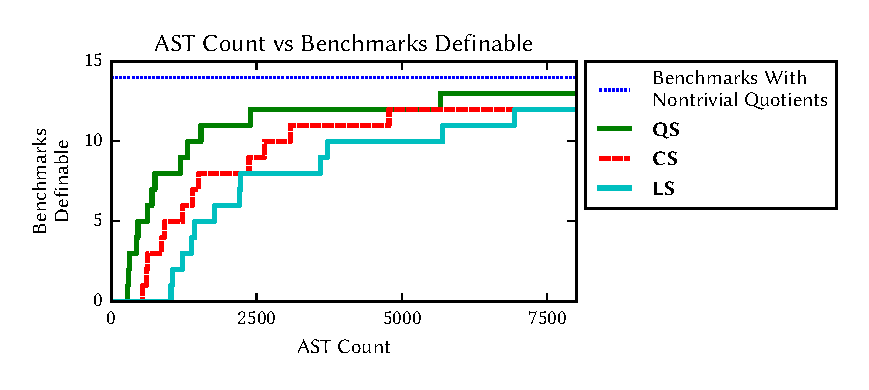
\includegraphics{generated-graphs/asts.eps}
\caption{Count of benchmark programs definable using a given AST count. We find
that it takes far fewer AST nodes to define benchmark lenses using QRE
synthesis than with Optician without QRE synthesis or without synthesis.}
\label{fig:asts}
\end{figure}

To get a sense of how much the new expressiveness that combining QRE lenses with
synthesis saves in terms of programmer effort, we compared the amount of code
that would need to be written for each of the lens benchmarks. We use number of
nodes in the abstract syntax tree as a measure of code size, and calculated
three quantities for each lens synthesis benchmark task. We only compared the
sizes on benchmarks where the canonization functions are nontrivial.
%
\begin{itemize}
  \item[\QRESize{}] the number of AST nodes in the QRE
  specifications (including examples).
  \item[\canonizeAndSpecSize{}]  the number of
  AST nodes in $W(q_1)$ summed with the number of AST nodes in $\canonize(q_1)$
  and the number of examples.
  \item[\LensAndSpecSize{}] the number of AST nodes
  in $W(q_1)$ summed with the number of AST nodes in the synthesized QRE lens.
\end{itemize}

The value of \QRESize{} is our measure of the programmer burden for
writing our benchmarks---it measures the number of AST nodes the programmer has
to write using the full expressiveness of QREs and synthesis.

The value of \canonizeAndSpecSize{} estimates the burden for writing our
benchmarks within the Optician system, without QREs but still using
synthesis. (This is only an approximation, as both $W(q_1)$ and $\canonize(q_1)$ are
automatically generated from the QRE, and it is possible that a human-written
version might be smaller.)

The value of \LensAndSpecSize{} estimates the burden in writing our benchmarks
in Boomerang, using neither QREs nor synthesis. (This is also an
approximation, as $W(q_1)$ and $\canonize(q_1)$ and the bijective lens are all
automatically generated.)

Figure~\ref{fig:asts} shows the number of benchmarks that can be expressed using
at most a given number of AST nodes. On average, \canonizeAndSpecSize{} used
44\% more AST nodes than \QRESize{}, using an average of 237 more AST nodes. On
average, \LensAndSpecSize{} used 193\% more AST nodes than \QRESize{}, using an
average of 1267 more AST nodes. This suggests that introducing QREs saves
programmers significant effort compared to both pre-QRE Optician and basic
Boomerang.

\subsection{Maintaining Competitive Performance}

\begin{figure}[t]
\centering
\begin{subfigure}[b]{.49\textwidth}
\centering
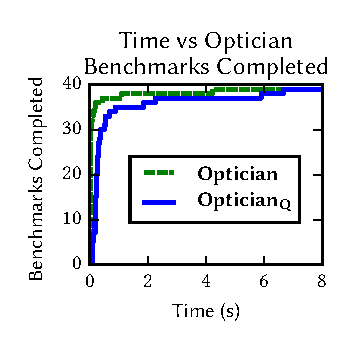
\includegraphics{generated-graphs/times_opt}
\caption{}
\label{subfig:lenssize}
\end{subfigure}
\begin{subfigure}[b]{.49\textwidth}
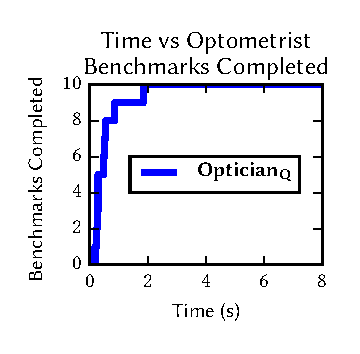
\includegraphics{generated-graphs/times_new.eps}
\caption{}
\label{subfig:examplesused}
\end{subfigure}
\caption{Runtimes of Optician and our system. In (a), we run Optician and our
  system on Optician's benchmarks. We find that there is only a negligible
  performance overhead incurred by using QREs. In (b), we run Optician with QREs
  on the Optician benchmarks we modified to use QREs. We find that it is able to
  synthesize all quotient lenses in under 20 seconds, and typically finished in
  under 5 seconds.}
\label{fig:times}
\end{figure}

To assess the performance impact of adding QRE support to Optician, we measured
the running time of the following configurations:
\begin{itemize}
  \item[\OpticianRuntime{}] pre-QRE Optician running on its own benchmarks.
  \item[\SystemOnOptician{}] Optician with QREs running on the pre-QRE
    benchmarks.
  \item[\SystemOnBenchmarks{}] Optician with QREs running on the benchmarks that
    were altered from Optician to include quotients.
\end{itemize}

We summarize the results of these experiments in Figure~\ref{fig:times}.  The
new version of Optician was able to synthesize all of pre-QRE Optician's
benchmarks at a speed competitive with the old version.  There is a small amount
of additional overhead introduced by QREs when calculating $W(q_1)$ and $K(q_1)$,
resulting in a very slight decrease in performance.

\section{Related Work}
\label{relwork}
This paper builds on the work of Foster et al~\cite{quotientlenses} who
introduced the theory of quotient lenses and implemented quotient lenses as a
refinement of the bidirectional string processing language
Boomerang~\cite{boomerang}. As we mentioned in
Section\cref{subsec:well-formed-qres}, all our QRE combinators can be expressed
using just the {\em normalize} combinator, which is one of the canonizer
primitives that Boomerang already supports. Also, all our QRE lens combinators
are already supported in Boomerang. Consequently Boomerang quotient lenses are
at least as expressive as our language of QRE lenses. 

Boomerang's canonizers allow one to canonize a regular language $R$ to by
mapping it to another regular language $S$ which may not be contained in $S$.
Formally, given sets $C$ and $B$ and an equivalence relation on $B$, Foster et
al defined a {\em canonizer} $q$ from $C$ to $B/{\sim_B}$ to be a pair of
functions $q.\kw{canonize} : C \longrightarrow B$ and $q.\kw{choose} : B
\longrightarrow C$ such that for every $b \in B$,
$$q.\kw{canonize} \; (q.\kw{choose} \; b) \sim_B \; b$$
This definition gives allows much more latitude for defining canonizers than
QREs. For example, if $\sim_B = \kw{Tot}(B)$, the equivalence relation that
relates every element in $B$ to every other element in $B$, then every function
from $C$ to $B$ is a canonizer.

Because of this extra elbow-room, Boomerang has two primitive {\em duplication}
quotient lenses, the first of which can be derived using the following inference
rule,
\begin{prooftree}
\AxiomC{$\ell : C/{\sim_C} \Leftrightarrow A_1/{\sim_{A_1}}$}
\AxiomC{$f : C \longrightarrow A_2$}
\AxiomC{$A_1 \cdot^! A_2$}
\AxiomC{$\sim_A = \sim_{A_1} \cdot \kw{Tot}(A_2)$}
\QuaternaryInfC{$\kw{dup}_1 \ell \; f \; : \; C/{\sim_C} \Longrightarrow A_1
\cdot A_2/{\sim_A}$}
\end{prooftree}
\begin{align*}
(\kw{dup}_1 \; \ell \; f).\get \; c &= (\ell.\get \; c) \cdot (f \; c)\\
(\kw{dup}_1 \; \ell \; f).\lput \; (a_1 \cdot a_2) \; c &= \ell.\lput \; a_1 \; c\\
(\kw{dup}_1 \; \ell \; f).\create \; (a_1 \cdot a_2) &= \ell.\create \; a_1
\end{align*}
wiht the symmetric $\kw{dup}_2$ combinator discarding the first copy instead of
the second in the \lput/\create{} direction. 

Boomerang's more general definition for canonizers also allows quotient lenses
to be used as canonizers by using the taking the \kw{canonize} function to be
the \get{} component of a lens and the \kw{choose} function to be its \create{}
component. Naturally, QREs also take advantage of this ability to use lenses as
canonizers by allowing for user-defined functions to be used by the \kw{squash}
and \kw{normalize} combinators. Moreover, the added functionality of
synthesizing lenses further makes it easier to define canonizers, as well as
lenses.

Foster et al also discuss other bidirectional programming languages that
support quotienting of data including XSugar~\cite{xsugar}, biXid~\cite{bixid}
and X/Inv~\cite{Hu2004,Mu2004,Mu2006}; we refer the reader to the related work
section in \cite{quotientlenses} for this discussion.

Another language which supports quotenting is BiFluX~\cite{pacheco2014biflux}, a
bidirectional functional update language for XML. BiFluX is inspired by
the FLUX XML update language~\cite{cheney2008flux}, and adopts a bidirectional
programming by update paradigm, where a program succintly and precisely
describes {\em how} to update a source document with a target document, in an
intuitive way, such that there is a unique ``inverse'' source query for each
update program. The source and view types of BiFluX programs are given by
regular expressions.

In BiFluX, a regular expression $R$ is said to be unambiguous if there is only
one way to parse a {\em flat} value of type $R$ to a stuctured value of type
$R$; here a flat value of $R$ is a value of $R$ with all left/right tags,
parantheses and list brackets removed. The bidirectional part of BiFluX involves
transforming source regular expressions to view regular expressions so that
data sequences described by the two types can be matched. This process can
result in intermediate types that are unambiguous, and this ambiguity can cause
unintended updates to be made the source, especially when information is
discared in this process. The typechecking phase of a BiFluX program therefore
includes a {\em type normalization} phase that tries to normalize a source types
using automata reduction techniques, and derive a lens between ambiguous and
unambiguous types. On the view side, this phase only tries to normalize view
types into isomorphic types.

{\em Formlenses}~\cite{rajkumar2014lenses} are a variant of lenses that perform
transformations up to equivalence. Formlenses are a bidirectional generalization
of {\em formlets}~\cite{cooper2008essence}. Formlets are a high-level
abstraction for building Web forms, and can be represented in Haskell as
functions that take a source of names---concretely, an \kw{Int}---as an
argument and produce a triple consisting of an HTML document, a {\em collect}
function, and a modified namesource:
\begin{center}
\begin{lstlisting}
type Formlet a = Int -> (Html, Env -> a, Int)
\end{lstlisting}
\end{center}
The names of any generated form fields are drawn from the namesource, and the
{\em collect} function looks up precisely these names.
Rajkumar et. al. observe that formlets are a useful
abstraction, but they only address one half of the problem---they make it easy
to construct a function that {\em produces} a value of type \kw{a}, but they do
not provide a way to describe a function that {\em consumes} a value of type
\kw{a} and embeds it in a form. A different way to think about this problem is
to observe that forms are often used to present an {\em updateable view} of the
data source. Therefore, Rajkumar et. al. leverage the power of bidirectional
transformations to define formlets that behave like updatable views, yielding
the abstraction of formlenses.

They \kw{Formless} type is given by,
\begin{center}
\begin{lstlisting}
type Formlens a = Maybe a -> [Int] -> (Html,Env -> Maybe a,[Int])
\end{lstlisting}
\end{center}
with the differences between this definition and the standard definition for
formlets being an extra \kw{Maybe a} parameter that provides an optional initial
value of the form, the namesource being changed to a list of integers, and the
{\em collect} function being allowed to return an optional value.

Rajkumar et. al. consider only formlenses that are well-formed in that a
well-formed formlens should only draw names from the namesource provided as an
argument, and the {\em collect} function should only look up corresponding
names.
Under this assumption, Rajkumar et. al. define what it means for a formlens to
be well behaved by defining a version of the classical GETPUT and PUTGET laws
for formlenses. These laws hold modulo an equivalence relation on environments,
since a formlens may be invoked with two separate namespaces, but this should
not affect the value stored in the information encapsulated in the type $a$.
Consequently, the GETPUT and PUTGET laws defined for formlenses are in spirit
analogous to the GETPUT and PUTGET laws for quotient lenses, since they hold up
to renaming of environment variables.

\iffalse
Well-behaved formlenses satisfy properties that are analogous to the classical
GETPUT and PUTGET law. If {\em extract} is a function from \kw{Html} to \kw{Env} that
extracts an environment containing the names and values of all the form fields
from an HTML document, then a formlens $f$ satisfies the Acceptability law if
for any $v$ of type $a$, $n$ of type \kw{Int} and environment $e$ of type
\kw{Env} if $f$ applied to \kw{Just v} and $n$ yields an HTML file $h$ and a
{\em collect} function $c$ where \kw{extract h} is contained in $e$, then
collect $e$
\fi

Finally, in Cunha~\cite{cunha2010relational} uses relational algebra to
encompass many of the existing approaches to bidirectional programming. For
example, using $\cdot$ to express relational composition, the GETPUT law states
that $\get \cdot \lput \subseteq \sim_V \cdot \pi_1$, where $\pi_1$ is the
projection onto the first factor. In addition to its generality, this
``point-free'' approach to defining bidirectional transformations has the
advantage of creating equational proofs of lens laws that proceed by folding
and unfolding combinator laws.

Now we turn to related work in synthesis. Much of the research in synthesis
assumes that the synthesizer is provided with a collection of examples.
Optician, as well as Optician enhanced with QREs for QRE lens synthesis, differ
in that they require that the programmer supplies both examples {\em and}
format descriptions in the form of regular expressions or QREs, though we are
far from the only ones to consider type-based synthesis.
There is a trade-off here.  On the one hand, a user must have some programming
expertise to write regular expression (or QRE) specifications, and it requires
some work. On the other hand, such specifications provide a great deal of
information to the synthesis system, which decreases the number of examples
needed (often to zero), makes the system scale well, and allows it to handle
large, complex formats.  By providing these format specifications, the 
synthesis engine does not have to both infer the format of the data as well as
the transformations on it, obviating the need to infer tricky formats like
those involving nested iterations. Furthermore, by focusing on bidirectional
transformations, we limit the space of synthesized functions to bijective ones,
reducing the search space, and the expressiveness of the search space.

There are many other recent results showing how to synthesize functions from
type-based
specifications~\cite{augustsson-2004,osera+:pldi15,feser-pldi-2015,scherer-icfp-2015,frankle+:popl16,armando+:pldi16}.
These systems enumerate programs of their target language, orienting their
search procedures to process only terms that are well-typed.
Optician is distinctive in that it synthesizes terms in a language with many
type equivalences.
Perhaps the system most similar to Optician is InSynth~\cite{gvero-pldi-2013}, a
system for synthesizing terms in the simply-typed lambda calculus that addresses
equivalences on types. Instead of trying to directly synthesize terms of the
simply-typed lambda calculus, InSynth synthesizes a well-typed term
in the succinct calculus, a language with types
that are equivalent ``modulo isomorphisms of products and
currying''~\cite{gvero-pldi-2013}. The type structure that we used in Optician
is significantly more complex.  In particular, because Optician types do not
have full canonical forms, we used a pseudo-canonical form, which captures part
of the equivalence relation over types. To preserve completeness, we pushed
some of the remaining parts of the type equivalence relation into a set of
rewriting rules and other parts into the synthesis algorithm itself.

Morpheus~\cite{morpheus} is another synthesis system that uses two
communicating synthesizers to generate programs.  In both Morpheus and
Optician, one synthesizer provides an
outline for the program, and the other fills in that outline with program
details that satisfy the user's specifications.
This approach works well in large search spaces that require some enumerative
search.
One important way that Optician differs from Morpheus is that in
Morpheus, an outline is a sketch---an
\emph{expression}
containing holes---whereas
an outline in Optician is a pair of regular
expressions, i.e., a
\emph{type}.  Moreover, in order to implement an efficient
search procedure, we had to create both a new type language and a new
term language for lenses.  Once we did so, we proved our new, more
constrained language
designed for synthesis was just as expressive as the original, more
flexible and compositional language designed for human programmers.

\section{Conclusion}
\bcp{And future work!}  \saz{I'm lukewarm about including a description of
future work.  Unless there are specific conjectures or open problems that
are worth mentioning, I'm not sure that it's really that important.}
\bcp{Agreed. But don't we have any ideas for how to extend or generalize or
things to do next or additional questions to consider??  E.g.: 
\begin{itemize}
\item is it easy to extend all this to
asymmetric and symmetric lenses?  (If so, we should say so!)
\item What properties do the bijective lens combinators have to have in
order to validate the normalization property?  (I.e., if we tried to extend
Boomerang's bijective lens combinators with another one, what would happen?)
\item Do we have more ideas for QRE primitives?
\item Etc.
\end{itemize}
}
\label{concl}

\bcp{Some of the citations need some love---e.g., the first one.}

\bibliographystyle{plain}
\bibliography{local}

\appendix
\addcontentsline{toc}{section}{Appendices}
\section*{Appendices}
\section{Proof of Normal Form Theorem for QRE lenses}
\cref{normal form} claims that if there is a derivation $q : Q_1
\Leftrightarrow Q_2$, then there exists a bijective lens $\ell : K(Q_1)
\Leftrightarrow K(Q_2)$ such that:
\begin{align*}
\llbracket q \rrbracket.\get &= \llbracket \ell \rrbracket\circ
\canonize(Q_1)\\
\llbracket q \rrbracket.\lput &= \llbracket \ell \rrbracket^{-1} \circ
\canonize(Q_2)
\end{align*}
We now prove this theorem.
\begin{proof}
We proceed by induction over the derivation $q : Q_1 \Leftrightarrow Q_2$.
\begin{enumerate}
  \item
  $\kw{lift}(\ell): R/\mathit{id}(R) \Leftrightarrow S/\mathit{id}(S)$ where
  $\ell : R \Leftrightarrow S$. Then
  \begin{align*}
\llbracket \kw{lift}(\ell) \rrbracket.\get &=  \llbracket \ell \rrbracket
= \llbracket \ell \rrbracket \circ id_{\mathcal{L}(R)} =
\llbracket \ell \rrbracket \circ \canonize(\mathit{id}(R)), \text{ and }\\
\llbracket \kw{lift}(\ell) \rrbracket.\lput &= \llbracket \ell
\rrbracket^{-1} = \llbracket \ell \rrbracket^{-1} \circ id_{\mathcal{L}(S)} =
\llbracket \ell \rrbracket^{-1} \circ \canonize(id(S))
\end{align*}
\item
$\lquot(Q_1, q): Q_1 \; ; \; Q_2 \Leftrightarrow Q_3$ where $q : Q_2
\Leftrightarrow Q_3$, $Q_1$ is well formed and $K(Q_1) = W(Q_2)$. Then
\begin{align*}
\llbracket \lquot(Q_1, q) \rrbracket.\get  &= \llbracket q
\rrbracket.\get \circ \canonize(Q_1)\\
\llbracket \lquot(Q_1, q) \rrbracket.\lput &= \llbracket q \rrbracket.\lput
\end{align*}
By the induction hypothesis, there exists a bijective lens $\ell :
K(Q_2) \Leftrightarrow K(Q_3)$ such that
\begin{align*}
\llbracket q \rrbracket.\get &= \llbracket \ell \rrbracket \circ
\canonize(Q_2)\\
\llbracket q \rrbracket.\lput &= \llbracket \ell \rrbracket^{-1} \circ
\canonize(Q_3)
\end{align*}
Consequently
\begin{align*}
\llbracket \lquot(Q_1, q)\rrbracket.\get  &= (\llbracket \ell \rrbracket \circ
\canonize(Q_2)) \circ \canonize(Q_1) = \llbracket \ell \rrbracket \circ
(\canonize(Q_1 \; ; \; Q_2))\\
\llbracket \lquot(Q_1, q) \rrbracket.\lput &= \llbracket \ell \rrbracket^{-1} \circ
\canonize(Q_3)
\end{align*}

\item
$\rquot(q, Q_3):Q_1 \Leftrightarrow Q_2 \; ; \; Q_3$ where $q : Q_1
\Leftrightarrow Q_2$, $Q_3$ is well formed and $K(Q_3) = W(Q_2)$. Proceed as in
the previous case.
\item
$q_1 \; ; \; q_2: c \Leftrightarrow Q_2$ where $q_1 : c \Leftrightarrow Q_1$ and
$q_2 : Q_1 \Leftrightarrow Q_2$. Then
\begin{align*}
\llbracket q_1 \; ; \; q_2 \rrbracket.\get &= \llbracket q_2
\rrbracket.\get\circ \llbracket q_1 \rrbracket.\get, \text{ and }\\
\llbracket q_1 \; ; \; q_2 \rrbracket.\lput &= \llbracket q_1 \rrbracket.\lput
\circ \llbracket q_2 \rrbracket.\lput
\end{align*}
By the induction hypothesis, there exist bijective lenses
$\ell_1 :
K(c) \Leftrightarrow K(Q_1)$ and $\ell_2 : K(Q_1) \Leftrightarrow K(Q_2)$ such
that
\begin{align*}
\llbracket q_1 \rrbracket.\get &= \llbracket \ell_1 \rrbracket \circ
\canonize(c)\\
\llbracket q_1 \rrbracket.\lput &= {\llbracket \ell_1 \rrbracket}^{-1} \circ
\canonize(Q_1)
\end{align*}
and
\begin{align*}
\llbracket q_2 \rrbracket.\get &= \llbracket \ell_2 \rrbracket \circ
\canonize(Q_1)\\
\llbracket q_2 \rrbracket.\lput &= {\llbracket \ell_2 \rrbracket}^{-1} \circ
\canonize(Q_2)
\end{align*}
Consequently,
\begin{align*}
\llbracket q_1 \; ; \; q_2 \rrbracket.\get &=
\llbracket q_2 \rrbracket.\get \circ \llbracket q_1 \rrbracket.\get \\
&=(\llbracket \ell_2 \rrbracket \circ \canonize(Q_1)) \circ (\llbracket \ell_1
\rrbracket \circ \canonize(c))\\
&= \llbracket \ell_2 \rrbracket \circ (\canonize(Q_1) \circ \llbracket \ell_1
\rrbracket) \circ \canonize(c)\\
&= (\llbracket \ell_2 \rrbracket \circ \llbracket \ell_1 \rrbracket) \circ
\canonize(c)\\
&= \llbracket \ell_1 \; ; \; \ell_2 \rrbracket \circ
\canonize(c)
\end{align*}
A similar argument shows that
$$\llbracket q_1 \; ; \; q_2 \rrbracket.\lput =
\llbracket \ell_1 \; ; \; \ell_2 \rrbracket^{-1} \circ
\canonize(c)$$
\item
$q^* : {Q_1}^* \Leftrightarrow {Q_2}^*$ where $q : Q_1 \Leftrightarrow Q_2$,
$W(Q_1)^{*!}$ and $W(Q_2)^{*!}$ and $K(Q_1)^{*!}$ and $K(Q_2)^{*!}$. Then
\begin{align*}
\llbracket q^* \rrbracket.\get &= (\llbracket q \rrbracket.\get)^*, \text{
and }\\
\llbracket q^* \rrbracket.\lput &= (\llbracket q \rrbracket.\lput)^*
\end{align*}
By the induction hypothesis there exists a bijective lens $\ell : K(Q_1)
\Leftrightarrow K(Q_2)$ such that
that
\begin{align*}
\llbracket q \rrbracket.\get &= \llbracket \ell \rrbracket \circ
\canonize(Q_1)\\
\llbracket q \rrbracket.\lput &= {\llbracket \ell \rrbracket}^{-1} \circ
\canonize(Q_2)
\end{align*}
Consequentlty
\begin{align*}
\llbracket q^* \rrbracket.\get &= (\llbracket \ell \rrbracket \circ
\canonize(Q_1))^* = \llbracket \ell \rrbracket^* \circ
\canonize(Q_1)^* = \llbracket \ell^* \rrbracket \circ
\canonize(Q_1^*)\\
\llbracket q^* \rrbracket.\lput &= (\llbracket \ell \rrbracket^{-1} \circ
\canonize(Q_2))^* = (\llbracket \ell \rrbracket^{-1})^* \circ
\canonize(Q_2)^* = \llbracket \ell^* \rrbracket^{-1} \circ
\canonize(Q_2^*)\\
\end{align*}
\item
$q_1 \cdot q_2: Q_1 \cdot Q_2 \Leftrightarrow Q_3 \cdot Q_4$, where $q_1 : Q_1
\Leftrightarrow Q_3 $,  $q_2 : Q_2 \Leftrightarrow Q_4$, $W(Q_1)
\cdot^! W(Q_2)$, $K(Q_1) \cdot^! K(Q_2)$, $W(Q_3) \cdot^! W(Q_4)$ and $
K(Q_3) \cdot^! K(Q_4)$. Then
\begin{align*}
\llbracket q_1 \cdot q_2 \rrbracket.\get &= \llbracket q_1 \rrbracket.\get \cdot
\llbracket q_2 \rrbracket.\get, \text{ and }\\
\llbracket q_1 \cdot q_2 \rrbracket.\lput &= \llbracket q_1 \rrbracket.\lput
\cdot \llbracket q_2 \rrbracket.\lput
\end{align*}
By the induction hypothesis, there exist bijective lenses $\ell_1 : K(Q_1)
\Leftrightarrow K(Q_3)$ and $\ell_2 : K(Q_2) \Leftrightarrow K(Q_4)$ such that
\begin{align*}
\llbracket q \rrbracket.\get &= \llbracket \ell_1 \rrbracket \circ
\canonize(Q_1)\\
\llbracket q \rrbracket.\lput &= {\llbracket \ell_1 \rrbracket}^{-1} \circ
\canonize(Q_3)
\end{align*}
and
\begin{align*}
\llbracket q_2 \rrbracket.\get &= \llbracket \ell_2 \rrbracket \circ
\canonize(Q_2)\\
\llbracket q_2 \rrbracket.\lput &= {\llbracket \ell_2 \rrbracket}^{-1} \circ
\canonize(Q_4)
\end{align*}
Consequently,
\begin{align*}
\llbracket q_1 \cdot q_2 \rrbracket.\get &= (\llbracket \ell_1 \rrbracket \circ
\canonize(Q_1)) \cdot  (\llbracket \ell_2 \rrbracket \circ
\canonize(Q_2))\\
&= (\llbracket \ell_1 \rrbracket \cdot \llbracket \ell_2
\rrbracket) \circ (\canonize(Q_1) \cdot \canonize(Q_2))\\
&= \llbracket \ell_1 \cdot  \ell_2 \rrbracket \circ \canonize(Q_1 \cdot Q_2)
\end{align*}
Similarly
$$
\llbracket q_1 \cdot q_2\rrbracket.\lput = \llbracket \ell_1 \cdot  \ell_2
\rrbracket^{-1} \circ \canonize(Q_3 \cdot Q_4) $$
\item
$\swap(q_1,q_2): Q_1 \cdot Q_2 \Leftrightarrow Q_4 \cdot Q_3$, where $q_1 : Q_1
\Leftrightarrow Q_3 $,  $q_2 : Q_2 \Leftrightarrow Q_4$, $W(Q_1)
\cdot^! W(Q_2)$, $K(Q_1) \cdot^! K(Q_2)$, $W(Q_4) \cdot^! W(Q_3)$ and $
K(Q_4) \cdot^! K(Q_3)$. Then
\begin{align*}
\llbracket \swap(q_1, q_2) \rrbracket.\get(s_1 \cdot s_2) &= \llbracket q_2
\rrbracket.\get(s_2) \cdot \llbracket q_1 \rrbracket.\get(s_1), \text{ and }\\
\llbracket \swap(q_1, q_2) \rrbracket.\lput(t_1, t_2) &= \llbracket q_1
\rrbracket.\lput(t_1) \cdot \llbracket q_2 \rrbracket.\lput(t_2)
\end{align*}
By the induction hypothesis, there exist bijective lenses $\ell_1 : K(Q_1)
\Leftrightarrow K(Q_3)$ and $\ell_2 : K(Q_2) \Leftrightarrow K(Q_4)$ such that
\begin{align*}
\llbracket q_1 \rrbracket.\get &= \llbracket \ell_1 \rrbracket \circ
\canonize(Q_1)\\
\llbracket q_1 \rrbracket.\lput &= {\llbracket \ell_1 \rrbracket}^{-1} \circ
\canonize(Q_3)
\end{align*}
and
\begin{align*}
\llbracket q_2 \rrbracket.\get &= \llbracket \ell_2 \rrbracket \circ
\canonize(Q_2)\\
\llbracket q_2 \rrbracket.\lput &= {\llbracket \ell_2 \rrbracket}^{-1} \circ
\canonize(Q_4)
\end{align*}
Consequently,
\begin{align*}
\llbracket \swap(q_1, q_2) \rrbracket.\get(s_1 \cdot s_2) &= \llbracket q_2
\rrbracket.\get(s_2) \cdot \llbracket q_1 \rrbracket.\get(s_1)\\
&= (\llbracket \ell_2 \rrbracket \circ
\canonize(Q_2))(s_2) \cdot  (\llbracket \ell_1 \rrbracket \circ
\canonize(Q_1))(s_1)\\
&= (\llbracket \swap(\ell_1, \ell_2) \rrbracket) \circ (\canonize(Q_1) \cdot
\canonize(Q_2)) (s_1, s_2)
\end{align*}
Similarly
$$
\llbracket \swap(q_1, q_2) \rrbracket.\lput = (\llbracket \swap(\ell_1, \ell_2)
\rrbracket)^{-1} \circ (\canonize(Q_4) \cdot \canonize(Q_3))$$
\item
$q_1 = q_1 \sep q_2$ where $q_1 : Q_1 \Leftrightarrow Q_3 $, $q_2 : Q_2
\Leftrightarrow Q_4$, $\mathcal{L}(W(Q_1)) \cap \mathcal{L}(W(Q_2)) =
\varnothing$ and $\mathcal{L}(W(Q_3)) \cap \mathcal{L}(W(Q_4)) = \varnothing$.
Then
$$
\llbracket q_1 \sep q_2 \rrbracket.\get(s) =
\begin{cases}
\llbracket q_1 \rrbracket.\get (s) & \text{if } s \in \mathcal{L}(W(Q_1))\\
\llbracket q_2 \rrbracket.\get (s) & \text{if } s \in \mathcal{L}(W(Q_2))\\
\end{cases}$$
$$\llbracket q_1 \sep q_2 \rrbracket.\lput(s) =
\begin{cases}
\llbracket q_1 \rrbracket.\lput (s) & \text{if } s \in \mathcal{L}(W(Q_3))\\
\llbracket q_2 \rrbracket.\lput (s) & \text{if } s \in \mathcal{L}(W(Q_4))\\
\end{cases}
$$
By the induction hypothesis, there exist bijective lenses $\ell_1 : K(Q_1)
\Leftrightarrow K(Q_3)$ and $\ell_2 : K(Q_2) \Leftrightarrow K(Q_4)$ such that
\begin{align*}
\llbracket q_1 \rrbracket.\get &= \llbracket \ell_1 \rrbracket \circ
\canonize(Q_1)\\
\llbracket q_1 \rrbracket.\lput &= {\llbracket \ell_1 \rrbracket}^{-1} \circ
\canonize(Q_3)
\end{align*}
and
\begin{align*}
\llbracket q_2 \rrbracket.\get &= \llbracket \ell_2 \rrbracket \circ
\canonize(Q_2)\\
\llbracket q_2 \rrbracket.\lput &= {\llbracket \ell_2 \rrbracket}^{-1} \circ
\canonize(Q_4)
\end{align*}
Consequently,
$$
\llbracket q_1 \sep q_2 \rrbracket.\get(s) =
\begin{cases}
\llbracket \ell_1 \rrbracket \circ
\canonize(Q_1) (s) & \text{if } s \in \mathcal{L}(W(Q_1))\\
\llbracket \ell_2 \rrbracket \circ
\canonize(Q_2) (s) & \text{if } s \in \mathcal{L}(W(Q_2)),\\
\end{cases}$$
so $\llbracket q_1 \sep q_2 \rrbracket.\get = \llbracket \ell_1 \sep
\ell_2 \rrbracket \circ \canonize(Q_1 \sep Q_2)$. A similar argument shows
that $\llbracket q_1 \sep q_2 \rrbracket.\lput = \llbracket \ell_1 \sep
\ell_2 \rrbracket^{-1} \circ \canonize(Q_3 \sep Q_4)$.\\
This completes the proof. 
\end{enumerate}
\end{proof}

\section{Proof of Correctness of \textproc{SynthQRELens}}
Theorem~\ref{thm:alg-correct} states that
  Given QREs $Q_1$ and $Q_2$, and a set of examples
  $\{(x_1,y_1),\ldots,(x_n,y_n)\}$, if there is a QRE lens $q : Q_1
  \Leftrightarrow Q_2$ such that $q.\get(x_i) \equiv_{Q_2} y_i \text{ and }
q.\lput(y_i) \equiv_{Q_1} x_i$, then $\textproc{SynthQRELens}(Q_1,Q_2,exs)$ will
return such a lens.  We prove that here.

\begin{lemma}[Algorithm Soundness]
  If $q = \textproc{SynthQRELens}(Q_1,Q_2,exs)$, then $q : Q_1 \Leftrightarrow
  Q_2$ and $q.\get(x_i) \equiv_{Q_2} y_i$  and 
$q.\lput(y_i) \equiv_{Q_1} x_i$ for all $(x_i,y_i)\in exs$.
\end{lemma}
\begin{proof}
  As $q = \textproc{SynthQRELens}(Q_1,Q_2,exs)$, we know that $q =
  \rquot(\lquot(Q_1, \ell), Q_2)$. Furthermore, we know that $\ell =
  \Call{SynthBijectiveLens}{R_1,R_2,exs'}$, where $exs' = \Call{Map}{exs,fun \,
    (ex_l,ex_r) \to (\canonize(Q_1)(ex_l),\canonize(Q_2)(ex_r))}$. By the correctness of
  $\textproc{SynthBijectiveLens}$, we know that $\ell.\get(x_i') = y_i'$ and
  $\ell.\lput(y_i') = x_i'$ for all $(x_i',y_i')\in exs'$. By definitions of
  $\rquot$ and $\lquot$, this means that:\\
$\rquot(\lquot(Q_1, \ell),
  Q_2).\get(x_i)$\\
 = $\ell.get(\canonize(Q_1)(x_i))$\\ $= \ell.get(x_i') = y_i' =
  \canonize(Q_2)(y_i) \equiv_{Q_2} y_i$ and\\
\\
$\rquot(\lquot(Q_1, \ell),
  Q_2).\lput(y_i)$\\
 = $\ell.\lput(\canonize(Q_2)(y_i))$\\ $= \ell.\lput(y_i') = x_i' =
  \canonize(Q_1)(x_i) \equiv_{Q_1} x_i$ as desired.
\end{proof}

\begin{lemma}[Algorithm Completeness]
  If there exists a QRE lens $q : Q_1 \Leftrightarrow Q_2$ such that
  $q.\get(x_i) \equiv_{Q_2} y_i$ and $q.\lput(y_i) \equiv_{Q_1} x_i$ for all
  $(x_i,y_i)\in exs$, then $\textproc{SynthQRELens}(Q_1,Q_2,exs)$ terminates.
\end{lemma}
\begin{proof}
  By Theorem~\ref{normal form}, there exists a bijective lens $\ell : K(Q_1)
  \Leftrightarrow K(Q_2)$, such that $q' = \rquot(\lquot(Q_1, \ell), Q_2)$ is
  semantically equal to $q$.

  This means that $q'.\get(x_i) \equiv_{Q_2} y_i$ and $q'.\lput(y_i)
  \equiv_{Q_1} x_i$ for all $(x_i,y_i)\in exs$. Unfolding the definitions of
  $\rquot$ and $\lquot$, we get:\\
  $q'.\get(x_i) = \ell.\get(\canonize(Q_1)(x_i)) = \canonize(Q_2)(y_i)$ and\\
  $q'.\lput(y_i) = \ell.\lput(\canonize(Q_2)(y_i)) = \canonize(Q_1)(x_i)$ for all
  $(x_i,y_i)\in exs$.

  By correctness of $\textproc{SynthBijectiveLens}$, we know that
  $\Call{SynthBijectiveLens}{R_1,R_2,exs'}$ terminates, so the entire algorithm
  terminates. 
\end{proof}

With soundness and completeness, we trivially get the correctness theorem.

\end{document}
